%%%%%%%%%%%%%%%%%%%%%%%%%%%%%%%%%%%%%%%%%%%%%%%%%%%%%%%%%%%%%%%%%%%%%%%%%%%%%%%%%%%%%%%%%%%%%%%%%%%%%
% This template is distributed with ABSOLUTELY NO WARRANTY.
% It serves as a guideline and constitutes a basic structure for a
% thesis/dissertation. The user assumes full responsibility for formatting
% and typesetting their document and for verifying that all the thesis
% requirements set by the University of Tennessee are met. Please refer to the most
% recent UT thesis guide (http://gradschool.utk.edu/thesesdissertations/formatting/)
% or contact the thesis consultant (http://gradschool.utk.edu/thesesdissertations/).
% Please report any bugs to the thesis consultant.
%%%%%%%%%%%%%%%%%%%%%%%%%%%%%%%%%%%%%%%%%%%%%%%%%%%%%%%%%%%%%%%%%%%%%%%%%%%%%%%%%%%%%%%%%%%%%%%%%%%%%
% O P T I O N S:
% 1. thesis/dissertation
% 2. monochrome
% 3. all options provided by the report class
%%%%%%%%%%%%%%%%%%%%%%%%%%%%%%%%%%%%%%%%%%%%%%%%%%%%%%%%%%%%%%%%%%%%%%%%%%%%%%%%%%%%%%%%%%%%%%%%%%%%%
%First, is this a thesis or dissertation? Choose one by commenting out the one you don't need:
%\documentclass[thesis,letterpaper,12pt]{utthesis} % thesis
%\documentclass[dissertation,letterpaper,12pt]{utthesis} %dissertation
% some alternatives are:
\documentclass[thesis,monochrome,letterpaper,12pt]{utthesis} %thesis, monochrome text
\renewcommand{\baselinestretch}{1.5} 	 % line Spacing
%%%%%%%%%%%%%%%%%%%%%%%%%%%%%%%%%%%%%%%%%%%%%%%%%%%%%%%%%%%%%%%%%%%%%%%%%%%%%%%%%%%%%%%%%%%%%%%%%%%%%
% TO DO: FILL IN YOUR INFORMATION BELOW - READ THIS SECTION CAREFULLY
%%%%%%%%%%%%%%%%%%%%%%%%%%%%%%%%%%%%%%%%%%%%%%%%%%%%%%%%%%%%%%%%%%%%%%%%%%%%%%%%%%%%%%%%%%%%%%%%%%%%%
%\title{Transverse energy analysis of Au+Au collisions at $\sqrt{s_{NN}}$ = 7.7, 11.5, 19.6, 27, and 39 GeV through the use of identified particles spectra}	       	% title of thesis/dissertation
\title{Transverse energy analysis of Au+Au collisions at 7.7, 11.5, 19.6, 27, and 39 GeV through the use of identified particles spectra}
\author{Biswas Sharma}                			% author's name
\copyrightYear{2018}            				% copyright year of your thesis/dissertation
\graduationMonth{August}           				% month of graduation for your thesis/dissertation
\degree{Master of Science}	    			% degree: Doctor of Philosophy, Master of Science, Master of Engineering...
\university{The University  of Tennessee, Knoxville}	% school name
%%%%%%%%%%%%%%%%%%%%%%%%%%%%%%%%%%%%%%%%%%%%%%%%%%%%%%%%%%%%%%%%%%%%%%%%%%%%%%%%%%%%%%%%%%%%%%%%%%%%%
% LOAD SOME USEFUL PACKAGES. 
% No need to change anything here, although if you'd like to add packages you can do that here. Note that packages preloaded with the utthesis class are: amsmath,amsthm,amssymb,setspace,geometry,hyperref,and color
%%%%%%%%%%%%%%%%%%%%%%%%%%%%%%%%%%%%%%%%%%%%%%%%%%%%%%%%%%%%%%%%%%%%%%%%%%%%%%%%%%%%%%%%%%%%%%%%%%%%%

\usepackage{nomencl}                    % produces a nomenclature
\usepackage{float}                      % figure floats
\usepackage[numbers]{natbib}                     % this package allows you to link your references
\usepackage{graphicx}					% graphics package
\graphicspath{ {figures/}{figures/eps/}{figures/pdf/} }% specify the path where figures are located
\usepackage{fancyhdr}                   % fancy headers and footers
\usepackage{url}                        % nicely format url breaks
\usepackage[inactive]{srcltx}		 	% necessary to use forward and inverse searching in DVI
\usepackage{relsize}                    % font sizing hierarchy
\usepackage{booktabs}                   % professional looking tables
\usepackage[config, labelfont={bf}]{caption,subfig} % nice sub figures
\usepackage{mathrsfs}                   % additional math scripts
\usepackage[titletoc]{appendix}			% format appendix correctly
\usepackage{pdflscape}					% to produce landscape pages if necessary
\usepackage{afterpage}
%\usepackage{fontspec}					% devnagari font?

%\RequirePackage{lineno}
%\setlength{\linenumbersep}{6pt}
%\linenumbers

%%%%%%%%%%%%%%%%%%%%%%%%%%%%%%%%%%%%%%%%%%%%%%%%%%%%%%%%%%%%%%%%%%%%%%%%%%%%%%%%%%%%%%%%%%%%%%%%%%%%%%
% This section formats landscape pages properly with the correct page number.
% This code is only necessary when landscape pages are needed and can be left alone
%%%%%%%%%%%%%%%%%%%%%%%%%%%%%%%%%%%%%%%%%%%%%%%%%%%%%%%%%%%%%%%%%%%%%%%%%%%%%%%%%%%%%%%%%%%%%%%%%%%%%%

\fancypagestyle{mylandscape}{
	\fancyhf{} %Clears the header/footer
	\fancyfoot{% Footer
    \makebox[\textwidth][r]{% Right
      \rlap{\hspace{.75cm}% Push out of margin by \footskip
        \smash{% Remove vertical height
          \raisebox{4.87in}{% Raise vertically
            \rotatebox{90}{\thepage}}}}}}% Rotate counter-clockwise
  \renewcommand{\headrulewidth}{0pt}% No header rule
  \renewcommand{\footrulewidth}{0pt}% No footer rule
}


%%%%%%%%%%%%%%%%%%%%%%%%%%%%%%%%%%%%%%%%%%%%%%%%%%%%%%%%%%%%%%%%%%%%%%%%%%%%%%%%%%%%%%%%%%%%%%%%%%%%%
\begin{document}
    \pagenumbering{alph} % this is needed to clear certain issues with the hyperref package
    %
    \addToPDFBookmarks{0}{Front Matter}{rootNode} % create a root node named "Front Matter" in the pdf bookmarks
    \addToPDFBookmarks{1}{Title}{a} % add a pdf bookmark to the title page
    \makeTitlePage % make the title page.
    %
    \pagenumbering{roman}
    \setcounter{page}{2}
    %
    \makeCopyrightPage % make the copyright page
    %
%%%%%%%%%%%%%%%%%%%%%%%%%%%%%%%%%%%%%%%%%%%%%%%%%%%%%%%%%%%%%%%%%%%%%%%%%%%%%%%%%%%%%%%%%%%%%%%%%%%%%
%The dedication and acknowledgments are optional. If you wish not to include them, simply comment out both the "\addToPDF..." line and the "\include{...}" line for each.
%%%%%%%%%%%%%%%%%%%%%%%%%%%%%%%%%%%%%%%%%%%%%%%%%%%%%%%%%%%%%%%%%%%%%%%%%%%%%%%%%%%%%%%%%%%%%%%%%%%%%
    \addToPDFBookmarks{1}{Dedication}{b} % add a pdf bookmark to the dedication page
    \include{front-matter/dedication} % include the dedication

    \addToPDFBookmarks{1}{Acknowledgments}{c} % add a pdf bookmark to the acknowledgments page
    \include{front-matter/acknowledgments} % include the acknowledgments
    
    \addToPDFBookmarks{1}{Abstract}{e} % add a pdf bookmark to the abstract page
    \chapter*{Abstract}\label{ch:abstract}

This thesis presents an analysis of the transverse energy resulting from the collisions of gold nuclei at the Relativistic Heavy Ion Collider in Brookhaven National Laboratory. The transverse momentum distributions available from the STAR detector corresponding to nine different centralities for eight different identified particles, $\pi^\pm$ [pions, anti-pions], $K^\pm$ [kaons, anti-kaons], $\Lambda^\pm$ [lambdas, anti-lambdas], $p$ [protons], and $\bar{p}$ [anti-protons], resulting from the collisions at five different center-of-mass energies per nucleon -- 7.7, 11.5, 19.6, 27, and 39 GeV -- are used in the calculations of the corresponding transverse energies. The results, when compared with the calorimetric transverse energy measurement from the PHENIX detector, show discrepancies of up to 2.83 $\sigma$ [standard deviations].
 % your abstract

    \addToPDFBookmarks{0}{Table of Contents}{f}
    \tableofcontents % generate a table of contents
    \listoftables % generate a list of tables
    \listoffigures % generate a list of figures
   
    \newpage
    \pagenumbering{arabic}
    \setcounter{page}{1}
    %%%%%%%%%%%%%%%%%%%%%%%%%%%%%%%%%%%%%%%%%%%%%%%%%%%%%%%%%%%%%%%%%%%%%%%%%%%%%%%%%%%%%%%%%%%%%%%%%%%%%
    % INCLUDE THE CHAPTERS STARTING WITH THE NOMENCLATURE IF PRESENT
    %%%%%%%%%%%%%%%%%%%%%%%%%%%%%%%%%%%%%%%%%%%%%%%%%%%%%%%%%%%%%%%%%%%%%%%%%%%%%%%%%%%%%%%%%%%%%%%%%%%%%
    \include{front-matter}
    \chapter{Introduction} \label{ch:introduction}

%\section{A Brief History of the Universe}
The Big Bang model is based on observational evidence, such as the cosmic microwave background radiation and the cosmological expansion \cite{Scott:2005uf,Perlmutter:1998np}, and suggests that at the beginning the universe must have been at a state of extremely high density and temperature. As the universe expanded, it went through several stages of cooling characterized by the formation of matter with different compositions.% The matter we mostly observe today exists at temperatures and densities much lower compared to those in the early universe.

%\section{Production of Historical Matter}
The Large Hadron Collider (LHC) at CERN and the Relativistic Heavy Ion Collider (RHIC) at the Brookhaven National Laboratory have the ability to collide heavy nuclei, such as those of gold and uranium, at nearly the speed of light, reaching temperatures of trillions of degrees Celcius. These laboratories have provided evidence of the formation of an exotic state of matter, called the quark-gluon plasma (QGP) \cite{FOKA2016154,Gyulassy:2004vg}. It only exists for a brief amount of time after such collisions and instantly freezes out into a plethora of new particles, which carry the signatures we can use to deduct QGP properties. Its properties suggest that it should be similar to the matter that existed within microseconds of the genesis of the universe, about 13.8 billion years ago \cite{ADAMS2005102,2013ApJS..208...20B,2016A&A...594A..13P}.% It behaves like an almost perfect fluid with a viscosity near 0 

%\section{Motivation of This Thesis}
One of the methods to probe the properties of this matter is by analyzing the conversion of the beam-direction energy at the time of collision into transverse energy after the collision. These measurements can be used to estimate the energy density of the QGP. This analysis is generally done by using data from the calorimeters (section \ref{section:calorimeters}) placed around the collision site. In this thesis, I use the data collected by tracking detectors (section \ref{tracking}), instead of the conventional calorimeters, to calculate the transverse energy.

%\section{Organization of The Thesis}
This thesis is structured as follows. Chapter \ref{ch:background} briefly describes the theoretial background associated with the concept of the quark-gluon plasma. In chapter \ref{ch:RHI-collisions}, I summarize the experimental concepts pertaining to relativistic heavy-ion collisions and the production and detection of QGP. Chapter \ref{ch:measurement} consists of the formalism of the measurement of transverse energy using calorimeters as well as tracking detectors. It also describes what has been done using calorimeters. Chapter \ref{ch:analysis} describes the data used to perform the analysis in this thesis and notes the relevant details of the analysis. In chapter \ref{ch:results}, I present the results and compare them to the ones in literature obtained using a different method. Chapter \ref{ch:conclusion} concludes the thesis and discusses what can be done in the future using the results of and the software developed for this analysis.

    \chapter{Theoretical Background} \label{ch:background}

% \section{Quantum Chromodynamics}

% \section{Phase Transitions}

% \section{Quark-Gluon Plasma}

\section{Quantum Chromodynamics}\label{section:QCD}
%%%%%%%%%%%%%%%%%%%%%%%%%%%%%%%%%%%%%%%%%%%%%%%%%%%%%%%%%%%%%%%%%%%%%%%%%%%%%%%
The strong force is one of the four fundamental interactions in physics. At large scales, it is also known as the residual strong force, and it is responsible for binding the nucleons together to give the nucleus its structure. At smaller scales, it is called the fundamental nuclear force, and it binds the fundamental units of subnuclear matter, the quarks, together to form the nucleons. The force carriers of the interaction are the mesons at the former scale and the gluons at the latter. %The scales of the different interactions and their relative strengths are summarized in table \ref{table:forces}.......... 
The electrodynamic interaction between charged particles such as protons and electrons is described by quantum electrodynamics (QED) as mediated by photons; the strong interaction, albeit more complicated, is explained under the framework of quantum chromodynamics (QCD) \cite{KAPUSTA1979461, Shuryak1988}. The quarks and gluons of QCD are collectively known as partons. Gluons are the gauge bosons of the Yang-Mills theory.

The Yang-Mills theory is a non-Abelian gauge theory. It has a Lagrangian with several degrees of freedom, some of which are redundant and need to be gauged. This is done by a mathematical treatment as prescribed under a gauge theory \cite{aitchison2003gauge}. The gauge theory associated with the Yang-Mills theory is based on the SU(N) group. It is non-Abelian as represented by the non-commutative transformations. QCD is a gauge theory that describes the application of the SU(3) symmetry transformations on color charges, namely red, blue, and green. The electroweak theory, which describes the electromagnetic as well as nuclear weak interactions, can be formalized under the gauge group SU(2)$\times$U(1). Together, they form the SU(3)$\times$SU(2)$\times$(U1) gauge theory called the standard model.
%Along with electric charge, mass and spin, quarks have the intrinsic property of color charge. 

One of the ways QCD is different from QED is the confinement of partons. In QED, the fundamental particles are bound together by the Coulomb potential, which diminishes with distance between the charge-carrying particles, as demonstrated by the relation \ref{eqn:QED-potential}:
\begin{equation}\label{eqn:QED-potential}
V_{C}\propto\frac{1}{r} 
\end{equation}
where $V_{C}$ is the Coulomb potential, and $r$ is the spatial separation between the particles. This means that bound QED particles can be isolated by increasing their spatial separation. The QCD potential, on the other hand, has an extra linear term in it%:
%(pg 7 https://www2.ph.ed.ac.uk/~muheim/teaching/np3/lect-qcd.pdf)
%(pg 68 https://arxiv.org/pdf/hep-ph/0001312.pdf)
, which means that the potential increases linearly with distance at large distances, and so an infinite amount of energy is required to separate quarks \cite{Bali:2000gf}. Hence, we never observe isolated quarks and they are said to be confined, not just bound, to form composite structures called hadrons \cite{0954-3899-32-3-R01}. A quark and an anti-quark forms a meson and three quarks forms a baryon. In addition to having a color charge, a quark also carries a flavor. There are six different quarks based on the flavors they carry: up, down, top, bottom, beauty, and strange.

%QCD is a gauge theory. Its Lagrangian remains unchanged under certain transformations. The Lagrangian has a number of degrees of freedom, some of which are redundant and need to be gauged, meaning regulated by a particular mathematical treatment. That mathematical treatment, in which the transformations of the gauge group are non-commutative, is described by a non-Abelian gauge theory. The Yang-Mills theory is an example of it. In this theory, the gauge boson is the gluon. 
%These confined, bound states of quarks and gluons is color-neutral.
%, and it is ergonomically more favorable to create a quark-antiquark pair than to produce unbound quarks
%, and $\alpha\_{QED}$ is the coupling constant.

\section{Phase Transitions}
%%%%%%%%%%%%%%%%%%%%%%%%%%%%%%%%%%%%%%%%%%%%%%%%%%%%%%%%%%%%%%%%%%%%%%%%%%%%%%%%%%%%%%%%%%%%%%
In everyday life, we observe matter existing in four distinct phases: solid, liquid, gas, and plasma. Changes in physical conditions can lead to a transition from one of these phases to another, exemplified by the commonly observed conversion of ice to water. Distinctions among the various phases can be represented in a chart called the phase diagram.

The phase diagram consists of thermodynamic observables such as temperature and density on its axes. Curves in the phase diagram represent boundries of physical conditions separating one phase from another: crossing a boundary represents an abrupt transition from one phase to another. This abruptness is mathematically characterized by the discontinuity in the change of the derivative of the free energy -- a thermodynamic variable -- with respect to the physical quantities in the axes. Such an abrupt transition is called a first-order phase transition. Along the boundary represented by the curve, there can be a point beyond which the phase transition is continuous instead of being abrupt, and the distinction between two phases is not clear. This point is called a critical point, and the phase transition that takes place beyond this point is called a crossover.% .............. Christine believes this is only for a first order phase transition................ 

One of the main focuses of current experimental and theoretical nuclear physics research is the study of the phase diagram of strongly interacting matter at a range of temperatures and baryon chemical potentials. In experiments involving the collisions of heavy ions at high and low energies, different regions of the phase diagram can be probed by varying the collision energy \cite{PhysRevC.93.024901}. For instance, the high-baryon chemical potential regime corresponds to lower beam energies and higher temperatures correspond to higher beam energies. The results of these experiments and model calculations can be used to study the possibilities and signatures of transitions in the QCD phase diagram.

A schematic representing the QCD phase diagram as a function of the temperature (T) and quark chemical potential ($\mu$) is shown in Fig. \ref{fig:PhaseDiagram} \cite{1742-6596-761-1-012066}. A crossover is predicted at low baryon chemical potentials (close to baryon-antibaryon symmetry) and high temperatures reminiscent of the early universe. Methods to study this region of the phase space will be explored in this thesis. At low temperatures and high net baryon densities, loose predictions have been made regarding the existence of exotic phases of high density matter, and programs, such as the Compressed Baryonic Matter experiment at the Facility for Antiproton and Ion Research in Germany, are being designed to study this region of the phase diagram \cite{HEUSER2013941c}.
% but within reach at modern facilities, specifically the Relativistic Heavy Ion Collider (RHIC) at the Brookhaven National Laboratory and the Large Hadron Collider (LHC) at CERN
%Details about these facilities are given in \ref{section:RHI-collisions}.
\begin{figure}[tb]
  \centering
  \includegraphics[width=4.5in]{figures/1742-6596-761-1-012066.png}\\
  \caption{Schematic of the QCD phase diagram \cite{1742-6596-761-1-012066}.}\label{fig:PhaseDiagram}
\end{figure}


\section{Quark-Gluon Plasma}
%%%%%%%%%%%%%%%%%%%%%%%%%%%%%%%%%%%%%%%%%%%%%%%%%%%%%%%%%%%%%%%%%%%%%%%%%%%%%%%%%%%%%%%%%%%%%%
The confinement of quarks into the hadronic phase of QCD matter, as described in section \ref{section:QCD}, has its limitations. At very high densities, when the wave function of a single hadron overlaps with the spatial regions covered by multiple such hadrons, it is impossible to classify which pair or triplet of quarks belongs to which meson or baryon. As long as a particular quark is close enough to the other quarks in the volume, it is deconfined in such a way that it can freely move anywhere in the volume \cite{0954-3899-32-3-R01}. QCD predicts such phase transition, at energy densities above 0.2-1 GeV/fm$^{3}$ \cite{Adam:2139456} and around a critical temperature of about 160 MeV \cite{FLORIS2014103}, of strongly interacting matter to a phase with quarks and gluons in thermal and chemical equilibrium representing the relevant degrees of freedom. This deconfined state of quarks and gluons is termed the quark-gluon plasma (QGP) in analogy to the quantum electrodynamical plasma phase of matter. The QGP has been found to behave like an almost perfect fluid \cite{PhysRevLett.109.152303}.
%\cite{FLORIS2014103 better reference than 2013arXiv1304.1452M}
%The deconfinement is what the weakening of the strong interaction due to the polarization of the QCD vacuum is expected to lead to at high energies. The expectation of this phase transition also makes sense in terms of the chiral symmetry of the QCD Lagrangian, which is spontaneously broken at low temperatures, but restored at high temperatures, providing a sufficient condition for the deconfinement.
% Existence of QGP in the early universe
% Production of QGP in the lab

    % \chapter{Relativistic Heavy Ion Collisions}
% \section{RHIC and LHC}
% \section{Collision Energy and Geometry}
% \section{Kinematic Variables}
% \section{QGP Evolution}
% \section{Detection of Collision Products}
% \section{Detection of QGP Signatures}
% \subsection{Dilepton Production}
% \subsection{Bjorken Energy Density}
% \subsection{Collective Flow}
% \subsection{Strangeness Enhancement}
% \subsection{Jet Quenching}
% \subsection{Photon Production}
% \section{Transverse Energy}
% \section{RHIC Beam Energy Scan Program}

\chapter{Relativistic Heavy Ion Collisions}\label{ch:RHI-collisions}
%%%%%%%%%%%%%%%%%%%%%%%%%%%%%%%%%%%%%%%%%%%%%%%%%%%%%%%%%%%%%%%%%%%%%%%%%%%%%%%%%%%%%%%%%%%%%%
The experimental evidence for the QGP comes from the collisions of heavy nuclei. Some of its signatures are described in section \ref{section:signatures}. Physicists proposed the existence of such matter since as far back as 1984, when nuclei were accelerated and collided with stationary targets \cite{Gyulassy:2004vg}. They were able to agree on a conclusive discovery of this matter during the 2000s, after colliding accelerated nuclei with other such nuclei or smaller species (protons, deuterons) at unprecedented energies and with improved detection schemes \cite{Ritter:2004xj}. With further increases in collision energies and enhancements in detector technology, modern accelerator facilities provided additional evidence and estimates of some of the properties as well as the dynamics of the evolution of the QGP. The following sections describe two such facilities, the physics of the collisions, and what happens after the collisions.

\section{RHIC and LHC}
The Relativistic Heavy Ion Collider (RHIC) is located in Upton, New York in the premises of the Brookhaven National Laboratory (BNL). Its construction started in 1991 and was completed in 1999. Figure \ref{fig:RHIC_layout} shows the layout, at the time of construction, of the collider along with the Alternating Gradient Synchrotron (AGS) complex and the locations of the original four detectors: Solenoidal Tracker At RHIC (STAR), Pioneering High Energy Nuclear Interaction eXperiment (PHENIX), Phobos, and BRAHMS (Broad RAnge Hadron Magnetic Spectrometers). Phobos, BRAHMS, and PHENIX were decommissioned after the completion of their science objectives, but STAR is still operational. The AGS was part of BNL before the construction of the RHIC, and its capabilities were augmented with the construction of the AGS Booster in 1991.
\afterpage{%
\begin{figure}[h]
  \centering
  \includegraphics[width=6.5in]{figures/RHIC_Layout.jpeg}
  \caption{Initial layout of the RHIC \cite{doi:10.1093/ptep/ptu093}.}\label{fig:RHIC_layout}
\end{figure}
\clearpage
}
Heavy ion beams in RHIC are created in a series of steps before collision. In case of gold ions, a pulsed sputter source produces negatively charged ions, which are stripped of some of their electrons with a foil on the positive end of the high-voltage Tandem Van de Graff. The ions are now positively charged and are accelerated to 1MeV/u toward the negative terminal of the Tandem. Upon exiting it, some more stripping takes place. The bending magnets then selectively deliver +32 charge states of the ions to the Booster Synchrotron, which accelerates them to 95MeV/u and strips them to a +77 charge state before injecting them to the AGS. The AGS accelerates them to 10.8 GeV/u and strips them of the remaining two electrons at the exit. The gold ions are then injected through the AGS-to-RHIC Beam Transfer Line to the two RHIC rings. These rings carry beams moving in opposite directions and intersect at six symmetric locations in the 3.8 km circumference. The original four detectors are located in four of these six locations where the beams undergo head-on collisions.

The Large Hadron Collider (LHC) is located underground (between 45m and 170m) beneath the France-Switzerland border near the city of  Geneva. The two rings of the collider were constructed between 1998 and 2008 by the European Organization for Nuclear Research (CERN) in the 26.7 km circular tunnel originally housing CERN's Large Electron-Positron collider. Analogous to the RHIC, the LHC gets its beams prepared by a series of machines in the CERN accelerator complex. The collisions occur at the locations of the four big LHC experiments: Compact Muon Solenoid (CMS), A Toroidal LHC ApparatuS (ATLAS), Large Hadron Collider beauty (LHCb) experiment, and A Large Ion Collider Experiment (ALICE). ALICE is dedicated to the study of heavy-ion collisions \cite{1748-0221-3-08-S08001}.
%%%%%%%%%%%%%%%%%%%%%%%%%%%%%%%%%%%%%%%%%%%%%%%%%%%%%%%%%%%%%%%%%%%%%%%%%%%%%%%%%%%%%%%%%%%%%%%%

\section{Collision Energy and Geometry}\label{geometry}
What happens in the aftermath of a collision depends on how much energy is available at the time of the collision as well as the geometry of the collision. The collision energy is determined by the collider configuration. The geometry of the collision is deduced as the collision $centrality$, as described later in this section, through the estimation of the charged particle multiplicities ($N_{ch}$) resulting from the collisions.  

In collision experiments, it is convenient to use a reference frame in which the net momentum of the pair of colliding species is zero. This frame is called the center-of-mass frame. In this frame, the total energy of the species in the two beams is a function of the number of nucleons and the center-of-mass energy per nucleon. The collision energy is reported as the center-of-mass energy per nucleon pair, $\sqrt{s_{NN}}$. %The magnitude of this quantity constrains the species that can be produced from any collision.

%!!!!!!!!!!!!!!! Details in:
%1. https://arxiv.org/pdf/1604.02651.pdf
%2. http://www.phys.hawaii.edu/~teb/phys481l/relkin.pdf
%3. http://edu.itp.phys.ethz.ch/hs10/ppp1/PPP1_4.pdf

RHIC has the unique capability of colliding species at a range of energies spanning almost two orders of magnitude. Table \ref{table:RHIC_specs} lists the collision energies produced so far at RHIC for various collision systems. The LHC boasts the highest amount of collision energy for any collider on earth. It collided species (p+p, p+A, Pb+Pb) at a center of mass energy up to 2.76 TeV per nucleon pair at the end of 2010. At the end of 2015, 5.02 TeV Pb+Pb and 13 TeV p+p collisions were successfully completed \cite{FOKA2016154}.

\begin{table}[!b]
\centering
\caption{Colliding species and associated collision energies at RHIC \cite{McGlincheyPrivateCommunication}.}
\begin{tabular}{||c c||}
%\tabletypesize{\scriptsize}
%\rotate
\hline
Collision system & $\sqrt{s_{NN}}(GeV)$ \\ [0.5ex]
\hline
\hline
p+p & 200, 510 \\
d+Au & 19.6, 39, 62.4, 200 \\
Cu+Cu & 62.4 \\
Cu+Au &  200 \\
p+Au & 200 \\
$^3$He+Au & 200 \\
Au+Au & 7, 7.7, 9, 20, 62, 130, 200 \\ [1ex]
\hline
\end{tabular}
%\caption{Colliding species and associated collision energies at RHIC \cite{McGlincheyPrivateCommunication}.}
\label{table:RHIC_specs}
\end{table}


In general, any collision between two nuclei is not perfectly head-on. Some collisions are close to being head-on and are called central collisions. Some are glancing and are called peripheral collisions. %The amount by which a collision is central is quantitatively represented by a variable called centrality. 
By convention, 0\% is the centrality of a perfectly head-on collision and 100\% is that of the least head-on, i.e., the most peripheral collision. More central collisions generally produce more particles \cite{Connors:2017ptx}.

The centrality is estimated through a model-based correlation between $N_{ch}$ and the impact parameter, defined as the distance between the centers of the two nuclei at the time of their maximum overlap. The Monte Carlo based model, for instance, assumes that all nucleons travel in straight lines along the beam direction \cite{Loizides:2014vua} and that they collide if they overlap \cite{Miller:2007ri}. $N_{ch}$ is assumed to scale with the number of participants and the number of binary collisions. The distribution of this quantity is then fit to the data and the fraction of the overlap is estimated from the observed $N_{ch}$ value. 5\% of all collisions with the highest $N_{ch}$ values, for example, are then referred to as being 0-5\% central \cite{Connors:2017ptx}.
% In practice, each collision event is deducted to belong to a specific centrality bin. For instance, 0-5\% would be the centrality for an identified $N_{ch}$ value which would be the minimum charged particle multiplicity produced by at most 5\% of the total number of collisions. This identification of the $N_{ch}$ value is often acheived by using the a Glauber model \cite{Connors:2017ptx,Miller:2007ri}.

Figure \ref{fig:mid-central_collision} illustrates the aftermath of a mid-central collision, i.e, a collision in which about half of the volume of each of the nuclei intersects the other.%............. add brief discussion of Glauber model and STAR centrality determination.............
\afterpage{%
	\begin{figure}[h]
	  \centering
	  \includegraphics[width=4.5in]{figures/flow_elliptic_init_v4.pdf}
	  \caption{An illustration of a mid-central collision of two nuclei traveling in the z direction. The X-axis is parallel to the line joining the centers of the two nuclei at the time of collision \cite{Connors:2017ptx}.}\label{fig:mid-central_collision}
	\end{figure}






\begin{figure}[h]
  \centering
  \includegraphics[width=6.5in]{figures/part_spec_Vovchenko.png}
  \caption{An illustration of a collision consisting of participants (solid red) and spectators (open blue) within the colliding nuclei labeled A and B. $t_{c}$ denotes the time of maximum overlap of the two nuclei. The apparent narrowing of the volumes of the nuclei in the z-direction is due to Lorentz contraction \cite{PhysRevC.90.044907}.}\label{fig:part_spec}
\end{figure}
\clearpage
}

The collision of two nuclei can be modeled as collisions of the constituents that make up the nuclei. The nucleons that take part in the collisions and are called participants. The rest of the nucleons are known as spectators. Figure \ref{fig:part_spec} illustrates the distribution of participants and spectators in two colliding nuclei.% Expectedly, the number of participants is more in more central collisions.
%%%%%%%%%%%%%%%%%%%%%%%%%%%%%%%%%%%%%%%%%%%%%%%%%%%%%%%%%%%%%%%%%%%%%%%%%%%%%%%%%%%%%%%%%%%%%%%%

\section{QGP Evolution}
\afterpage{%
\begin{figure}[h]
  \centering
  \includegraphics[width=5.5in]{figures/LightCone1_color-crop_NThesis.pdf}
  \caption{Evolution of the QGP represented in a lightcone diagram. $\tau_{0}$ denotes the formation time of the QGP. $T_{c}$ is the critical temperature of the transition from the QGP to the hadron gas phase. $T_{ch}$ and $T_{fo}$ stand for the temperatures at, respectively, chemical freeze-out and thermal freeze-out \cite{Connors:2017ptx}.}\label{fig:lightcone}
\end{figure}
\clearpage
}
The evolution of the QGP is shown in a lightcone diagram in Fig. \ref{fig:lightcone} \cite{Connors:2017ptx}. The initial state of the colliding nuclei is not precisely known and is the topic of research for upcoming experiments. During the collision, the participants scatter off of each other while the spectators keep traveling almost unperturbed in their original direction. The immediate aftermath of a central collision of heavy ions at RHIC and LHC energies is the formation of a hot fireball. This fireball evolves in time to form a liquid-like medium of quarks and gluons. This medium attains a local equilibrium and remains in such a state, depending on the collision energy, for about 1-10 fm/c. This equilibrium is broken as the liquid QGP evolves by expanding and cooling to attain a density and temperature at which the medium undergos hadronization followed by a chemical freeze-out to form a hadron gas. The particle ratios are fixed after the chemical freeze-out. Collisions between the constituents of this gas become scant as it evolves with further expansion and cooling, and the hadrons undergo a thermal freeze-out to attain their final energies and momenta \cite{Connors:2017ptx}.

\section{Detection of Collision Products}\label{subsection:detection}
%%%The final state particles emit in all directions around the collision site. The symbol $\theta$ is used to denote the polar angle of the direction, i.e., the angle with respect to the beam axis, of a particle. However, it is more convenient to use a different quantity, called the rapidity, to describe the particle's direction.
Detectors are placed around the collision site to perform measurements on the final state particles emitting from the thermal freeze-out of the medium. These measurements typically include the reconstruction of the particle tracks, estimation of the the types of particles, and the momenta and energies they carry.

Generally, a tracking detector surrounds the collision site, and there are particle identifiers followed by calorimeters around it. A magnetic field is applied parallel to the beam direction around the collision site. Due to this orientation of the magnetic field, the spectators traveling parallel to it move roughly undeflected and the final state charged particles with components of velocity transverse to the beam axis get deflected around the beam axis with radius given by
\begin{equation}\label{eqn:larmor}
r = \frac{p_{T}}{qB},
\end{equation}
where $p_{T}$ is the transverse momentum of the particle, $q$ is its electric charge, and $B$ is the applied magnetic field.
Two kinds of detectors most relevant to this thesis, tracking detectors and calorimeters, are described in chapter \ref{ch:measurement}.

\section{Detection of QGP Signatures}\label{section:signatures}
%http://iopscience.iop.org/article/10.1088/0954-3899/25/3/013/meta, and: 

The existence and properties of the QGP in the aftermath of high-energy heavy-ion collisions can be probed using different techniques relevant to several theoretical characteristics of the medium. No signature can alone be used to claim the production of the QGP, and some of the probes, which should be interpreted together, are described below.


%Analyses of experimental results have thus far provided signatures of the formation of matter with partonic degrees of freedom at the early stages of the collisions. Such signatures include suppression of high monentum hadrons, known as jet quenching, because the QGP is nearly opaque to colored probes, and large azimuthal anisotropies, indicating that the medium is a liquid of quarks and gluons \cite{PhysRevC.96.044904}?????. %Experiments also reveal the initial energy density of this matter to be about two orders of magnitude larger than that of low energy nuclear matter -- comfortably more than the deconfinement phase transition critical density predicted by lattice QCD \cite{2005PrPNP..54..443J}.

%The state of the colliding nuclei before the collision at LHC and top RHIC energies has indications of being a Color Glass Condensate -- strongly interacting, weakly coupled highly coherent gluonic matter \cite{1742-6596-458-1-012024}. The characteristics of the initial states of these nuclei affect the partonic distributions within the nuclei and ultimately the products of the collision. The collision products are also affected by variables such as the initial energy and entropy densities of the partonic matter \cite{2005PrPNP..54..443J}.

%Different observables can be used to study different aspects of heavy ion collisions. The charged particle multiplicity, $\langle N_{ch} \rangle$, is a global variable that relates to the entropy production during the collision (analysis note). The transverse energy, $E_{T}$, a global variable related to $\langle N_{ch} \rangle$, provides information about the conversion of the initial beam-direction kinetic energy into energy flowing in the transverse direction after the collision. Together, the studies of the fluctuation of the $\langle N_{ch} \rangle$ and the $E_{T}$ pseudorapidity [footnote] density with respect to the beam energy and the collision centrality [footnote] help probe the characteristics of the initial conditions at the time of the collision. One can study, for instance, the distinctions between models based on quark participants against those based on nucleon participants [analysis note]. These quantities can also lead to the rough estimate of the initial energy density through the use of the Bjorken formula \cite{2012ARNPS..62..361M}:
%\ref{eqn:Bjorken}
%\begin{equation}\label{eqn:Bjorken}
%\epsilon \geq \frac{\frac{dE_{T}}{d\eta}}{\tau_{0}\pi R^{2}} = \frac{3}{2}\langle \frac{E_{T}}{N} \rangle \frac{\frac{dN_{ch}}{d\eta}}{\tau_{0}\pi R^{2}}
%\end{equation}
%The transverse energy and the charged particle pseudorapidity densities have conventionally been calculated by using the transverse energy measurements obtained from calorimeters. This thesis details the use of particle spectra, reported as $\frac{d^{2}N}{dydp_{T}}$, from Au+Au collisions at RHIC to calculate the same global variables and serve as a method to cross check the ones involving calorimeters.
\subsection{Bjorken Energy Density}
%mostly pg 271 to 275 in \cite{Wilde:2012wc}
In 1983, J.D. Bjorken\cite{PhysRevD.27.140} prescribed a formula to use the final state particles to estimate the initial energy density, $\epsilon_{0}$, in a nucleus-nucleus collision. With slight changes in the original formula, the energy density is estimated by:
	\begin{equation}\label{eqn:bjorken}
	\epsilon_{0} = \frac{1}{\tau_{0}A_{T}}\langle\frac{dE_{T}}{dy}\rangle,
	\end{equation}
where $\tau_{0}$ is the formation time of the QGP, $A_{T}$ is the transverse area of the intersection of the two nuclei, and $\langle\frac{dE_{T}}{dy}\rangle$ is the mean transverse energy per unit rapidity. $\tau_{0}$ is model-dependent and is normally estimated to be $~1 fm/c$. $A_{T}$ depends on the centrality of the collision and can be estimated using the Glauber model discussed earlier. $\langle\frac{dE_{T}}{dy}\rangle$ is found from the measurement of the transverse energy carried by the final state particles from the collision and is the central theme of this thesis. Details about it are in the following chapters.
The estimate of the initial energy density from the Bjorken formula is an underestimate of the maximum energy density because the measured $dE_{T}/dy$ is an average over the system as it undergoes expansion and cooling. It can be compared with the QCD prediction of the critical energy density \cite{Adam:2139456} to check if the results from a collision imply the achievement of the critical physical condition required for the phase transition \cite{2005PrPNP..54..443J}. Experiments show that ultra-relativistic heavy ion collisions are capable of producing energy densities comfortably higher than those predicted by QCD \cite{Adam:2139456}.
%Experiments reveal it to be about two orders of magnitude larger than that of low energy nuclear matter -- comfortably more than the deconfinement phase transition critical density predicted by lattice QCD \cite{2005PrPNP..54..443J}.

\subsection{Elliptic Flow}
The evolution of the medium produced in relativistic heavy ion collisions can be well described under the framework of relativistic hydrodynamics \cite{SCHENKE2017105,2014NuPhA.926...92S}. This description indicates the presence of a collective flow of a locally thermalized liquid. The angular distribution of the momenta of the final state particles emitted out of the collectively flowing system can be decomposed into a Fourier expansion in its azimuthal components. The second harmonic coefficient, $\nu_{2}(y,p_{T})$, of this decomposition characterizes what is known as the elliptic flow \cite{2001PhLB..503...58H}. The magnitude of the elliptic flow from a non-central collision represents the anisotropy in azimuthal momentum space of the thermalized post-collision system \cite{2011NJPh...13e5008S}.
%In normal matter, the speed of sound is generally more in solid than in liquid and more in liquid than in gas. This is because it its proportional to the ......
The elliptic flow of the medium, as a function of the momentum or the kinetic energy in the transverse direction, points towards quarks, rather than hadrons, being the relevant degrees of freedom in the QGP. Figure \ref{fig:v2Scaling1} shows $v_{2}$ as a function of the transverse momentum and the transverse kinetic energy for identified particles. The spectra scale consistently at lower values of both $p_{T}$ and $KE_{T}$. However, they branch out as mesons and baryons at higher values: $p_{T} \gtrsim 2 GeV/c and KE_{T} \gtrsim 1 GeV$. Figure \ref{fig:v2Scaling2}, on the other hand, is similar to Fig. \ref{fig:v2Scaling1}, with the exception that both the axes have quantities that are normalized by the number of quarks, $n_{q}$. In this case, the $KE_{T}$ spectra strongly exhibits a scaling which is more comprehensively consistent with the number of quarks than in case of Fig. \ref{fig:v2Scaling1}. This universal quark-number scaling can be interpreted as the degrees of freedom of the system being quark-like \cite{2007PhRvL..98p2301A}.
\afterpage{%
	\begin{figure}[tb]
	  \centering
	  \includegraphics[width=4.5in]{figures/v2Scaling1.png}
	  \caption{Minimum-bias Au+Au ($\sqrt{s_{NN}} = 200 GeV$) elliptic flow spectra for identified particles: (a) $v_{2}$ vs $p_{T}$ and (b) $v_{2}$ vs $KE_{T}$ \cite{2007PhRvL..98p2301A}.}\label{fig:v2Scaling1}
	\end{figure}
	
	\begin{figure}[tb]
	  \centering
	  \includegraphics[width=4.5in]{figures/v2Scaling2.png}
	  \caption{Minimum-bias Au+Au ($\sqrt{s_{NN}} = 200 GeV$) elliptic flow spectra for identified particles: (a) $\frac{v_{2}}{n_{q}}$ vs $\frac{p_{T}}{n_{q}}$ and (b) $\frac{v_{2}}{n_{q}}$ vs $\frac{KE_{T}}{n_{q}}$ \cite{2007PhRvL..98p2301A}.}\label{fig:v2Scaling2}
	\end{figure}
\clearpage
}
\subsection{Prompt and Thermal Photons}
Most of the photons observed after relativistic heavy ion collisions are the results of the decay of the neutral pion into two gammas. %The remaining photons can be divided into direct photons from hard scatterings, which can be calculated in perturbative QCD, and thermal photons.
When these photons are subtracted from the observations, the remaining photons are called direct photons \cite{PAQUET2016409}. These direct photons are produced within the fireball via different mechanisms as discussed below.
\begin{figure}[!b]
  \centering
  \includegraphics[width=6.5in]{figures/directPhotons.PNG}
  \caption{Feynman diagram representing the production of photons from quarks and gluons. $(a)$ and $(b)$ represent annihilation processes, whereas $(c)$ and $(d)$ represent Compton processes \cite{wong1994introduction}.}\label{fig:directPhotons}
\end{figure}

In the QGP, a quark and an antiquark can annihilate to produce a photon and a gluon. It is also possible for the pair to annihilate and produce two photons, but the probability of this process is smaller than the former by about two orders of magnitude. Furthermore, a quark (or an antiquark) can interact with a gluon to produce an antiquark (or a quark) and a photon, a process analogous to Compton scattering in QED. The photons produced from the hard scattering processes between the partons are called prompt photons, and their multiplicity scales with the number of binary collisions. Photons can also be produced due to scatterings of partons within the thermalized medium, and these photons are called thermal photons. The nature of the $p_{T}$ distribution is different in this case as the emission process mimics blackbody radiation. This difference helps distinguish these photons from the direct photons produced by partonic interactions. Just like the leptons described in the previous section, the photons produced in the QGP can only interact with the medium electromagnetically. Therefore, they undergo minimal scattering before being detected, and hence can be used to probe the thermodynamical state of the medium at the time of their creation \cite{wong1994introduction,PAQUET2016409,Wilde:2012wc}.

\subsection{Strangeness Enhancement}
% http://shodhganga.inflibnet.ac.in/bitstream/10603/37674/11/11_chapter%202.pdf
The interacting nuclei carry no net strangeness before colliding, and so an observation of strange and multi-strange particles after the collision can be used to probe the properties of the post-collision medium \cite{1742-6596-455-1-012005}. Strangeness can also be produced in hadron-hadron collisions. However, it is enhanced in nucleus-nucleus collisions \cite{Behera:2012eq}. This is interesting because it possibly indicates a restoration of chiral symmetry, which is a topic of ongoing research: in the zero baryon chemical potential limit, lattice QCD calculations reveal a transition of QCD matter between a phase with broken and one with restored chiral symmetry \cite{ refId0}. Chiral symmetry restoration has the implication of all the flavors of quarks losing their masses \cite{Sazdjian:2016hrz}. Hence, when chiral symmetry is restored, it is more feasible to produce strange quarks, for instance, which have higher masses than the light quarks, up and down, in a state of broken chiral symmetry. Chiral symmetry restoration is not the only possible reason for the production of many strange quarks. It is also feasible to produce strange quarks as long as the temperature of the system is above the strange flavor mass scale, and so it carries effects of the system temperature. This is exemplified by the ratio of the production of the strange kaons to that of the non-strange pions, which are the most abundant hadrons produced from nucleus-nucleus collisions: kaon yield increases more rapidly than pion yield does as the temperature increases \cite{wong1994introduction}.% This can be shown mathematically by treating the system as a hadron gas in thermal and chemical equilibrium that follows the Bose-Einstein distribution, but it is beyond the scope of this thesis

% https://arxiv.org/pdf/1612.04078.pdf
% more: https://indico.cern.ch/event/555216/contributions/2414536/attachments/1394348/2125058/Bratkovskaya_WWND-2017.pdf

\subsection{Jet Quenching}
A scattering event in which the participants transfer a large amount of their original momenta is called hard scattering. The products of the scatterings are called jets. %Ultimately, jets are what are recognized by a jet finder algorithm as jets. 
In heavy-ion collisions, most hard scatterings are the results of two partons from the opposite nuclei scattering off each other. These partons can lose their momenta by strongly interacting with the enhanced gluon fields in a QGP medium. Therefore, the properties of the jets, as carried by the final state hadrons, should be different for collisions that produce the QGP as compared to those that do not, and hence they can be used as signatures and probes of QGP. Figure \ref{fig:jets} illustrates the quenching of jets that have to travel long distances in the medium.

The nuclear modification factor, $R_{AA}$, is the ratio of the cross section for particle production in nucleus-nucleus collisions scaled by the number of binary nucleon-nucleon collisions divided by the cross section in proton-proton collisions.  It is shown in Fig. \ref{fig:Raa} for several different particle species, demonstrating substantial suppression of high momentum particles. This shows that the medium is nearly opaque to colored probes.

%Details about the forms of interaction of the hard partons with the QGP is beyond the scope of this thesis. 
%%Formalisms developed to study jet quenching due to radiative and collisional energy losses are detailed in \cite{2015IJMPE..2430014Q}. 
	\begin{figure}[!b]
	  \centering
	  \includegraphics[width=4.5in]{figures/jets.PNG}
	  \caption{Illustration of jet quenching. Two jets are produced from each of the hard scatterings occuring at the locations of the solid dots. Jets originating closer to the initial surface are more probable to propagate outside the medium, as shown. Jets opposite to them interact with the medium, losing their energy and resulting in bow front shock waves \cite{STOCKER2005121}.}\label{fig:jets}
	\end{figure}
	
\afterpage{%
	\begin{figure}[!h]
	  \centering
	  \includegraphics[width=6.5in]{figures/Raa.PNG}
	  \caption{$R_{AA}$ from PHENIX for direct photons \cite{Afanasiev:2012dg}, $\pi^0$ \cite{Adare:2008qa}, $\eta$ \cite{Adare:2010dc}, $\phi$ \cite{Adare:2015ema}, $p$ \cite{Adare:2013esx}, J/$\psi$ \cite{Adare:2006ns}, $\omega$ \cite{Adare:2011ht}, $e^{\pm}$ from heavy flavor decays \cite{Adare:2010de}, and $K^{\pm}$ \cite{Adare:2013esx}.  This demonstrates that colored probes (high-$p_{T}$ final state hadrons) are suppressed while electroweak probes (direct photons) are not at RHIC.}\label{fig:Raa}
	\end{figure}
\clearpage
}
%The interaction of the jets in the QGP medium can be in the form of gluon bremsstrahlung or parton collision.

\section{The Beam Energy Scan Program}
The RHIC, in 2010, started a multi-phase Beam Energy Scan (BES) program to study the QCD phase diagram. Between 2010 and 2011, during the exploratory phase I of the BES program, the collider provided Au+Au collisions at 7.7, 11.5 (not completed in PHENIX), 19.6, 27, and 39 GeV. Together with the data formerly collected by the RHIC at higher collision energies, BES phase I data can scan the interval from 450 MeV to 20 MeV in $\mu_{B}$ space \cite{1742-6596-455-1-012037, LUO201675}. One of the things that can be studied with the data associated with this region of the phase space is the possibility of a ``turn-off of new phenomena already established at higher RHIC energies"\cite{1742-6596-455-1-012037}. Results corresponding to the high-$\mu_{B}$ region might provide evidence of a first order phase transition, and possibly the critical point \cite{LUO201675}.
% (https://drupal.star.bnl.gov/STAR/starnotes/public/sn0493)

The manifestation of such phenomena might be in terms of the fluctuations or other properties of the post-collision system. One can, for instance, study the scaling of the energy density after the collision with the longidutional energy at the time of the collision, $\sqrt{s_{NN}}$, for which one needs to measure the transverse energy. This can be done in multiple ways using a detector like STAR or PHENIX that is made up of sub-systems such as the Time Of Flight (TOF) detectors, Time Projection Chambers (TPCs)/Time Expansion Chambers, and calorimeters. The next chapter describes the measurement of transverse energy using BES data from PHENIX calorimeters. Also, the next chapter and the ones after it contain the procedures and the results of the analysis of the BES data from STAR using the identified particle spectra.

%\section{Transverse Energy}
%\section{RHIC Beam Energy Scan Program}

    \chapter{Measurement of Transverse Energy} \label{ch:measurement}
%\Conventional method using calorimeters
%\ first the math: definitions 1.3, 1.4 from analysis note
%\ then the description of the instruments used to get the relevant variables:
%\ 		primarily STAR (reference 12 from analysis note), include PHENIX and CMS later if needed

%\ transition to:

%\Spectra from the BES program
%\ Beam Energy Scan program
%\ particle identification
%\ transverse momentum spectrum (using tracking detectors????)
%\ errors associated with the spectra

%\Getting ET estimates from the spectra for individual particles
%\ equations relating dET/dy etc. to the pT integral of d2N/(dydpT)
%\ extrapolation of spectra to cover regions not covered by the experiment
%\ using ET estimates for individual particles to estimate total ET and the assumptions involved
%\ analysis note pg 7: "In this new method, ET is measured from charged hardon tracks...
%\ and the measured ET is SCALED UP to correct for neutral energy which is not observed...
%\ in tracking detectors."
%\ essentially, what really needs to be made clear is how the "scaling up" is done, because...
%\ even conventionally, STAR "uses information from the tracking detectors to measure ET from...
%\ charged hadrons and the electromagnetic calorimeter to measure ET from electrons, photons...
%\ and neutral hadrons which dominantly decay to electromagnetic particles." (hybrid method)

This chapter indroduces the definitions of transverse energy, ways to measure it using different detectors, and particular examples for the detectors at the RHIC.

\section{Definition of Transverse Energy}
The transverse energy, $E_{T}$, from a collision can be defined as the sum of the transverse masses, $m_{T}$, of all the particles produced in the collision, i.e.,
\begin{equation}\label{eqn:ETDefTheory}
E_{T}\equiv\sum_{i}m_{T,i}
\end{equation}
with
\begin{equation}\label{eqn:mT}
m_{T}\equiv\sqrt{p_{T}^{2}+m^2}
\end{equation}
where $m$ is the rest mass of the particle and $p_{T}$ is its transverse momentum. Using this definition to calculate the $E_{T}$ requires perfect identification of all the particles. It has not been possible to do so in experiments, and so a more feasible, operational definition of $E_{T}$ is used. A commonly accepted definition in the case of calorimetric measurements is \cite{PhysRevC.89.044905, PhysRevLett.109.152303}:
\begin{equation}\label{eqn:ETDefSum}
E_{T} = \sum_{i}E_{i}\sin{\theta_{i}},
\end{equation}
\begin{equation}\label{eqn:dETdEta}
\frac{dE_{T}}{d\eta}=\sin{\theta}\frac{dE}{d\eta},
\end{equation}

where the index $i$ runs over all the particles going into a fixed solid angle for each event, $\theta$ is the polar angle, i.e, the angle with respect to the beam axis, $\eta$ is the pseudorapidity defined as 
\begin{equation}\label{eqn:pseudorap}
\eta\equiv-\ln\tan{\frac{\theta}{2}},
\end{equation}
and $E_{i}$ is the energy deposited in the calorimeter by the $i^{th}$ particle. $E_{i}$ is considered to be, by convention \cite{PhysRevC.71.034908}, the following
\begin{equation}\label{eqn:EiCaseByCase}
E_{i} = 
	\begin{cases}
	E_{i}^{tot}-m_{0} & \text{for baryons} \\
	E_{i}^{tot}+m_{0} & \text{for anti-baryons} \\	
	E_{i}^{tot} & \text{otherwise} \\
	\end{cases}
\end{equation}
%\ $E_{i}^{tot}$ - $m_{N}$ in case of baryons, $E_{i}^{tot}$ + $m_{N}$ in case of antibaryons, and the $E_{i}^{tot}$ in case of other particles, 
where $E_{i}^{tot}$ is the total energy of the $i^{th}$ particle defined canonically as
\begin{equation}\label{eqn:Etot}
E^{tot}\equiv\sqrt{p^{2}+m_{0}^2}
\end{equation}
and  $m_{0}$ is the particle's rest mass.

$E_{i}$ given by equation \ref{eqn:EiCaseByCase} is what would be observed by a calorimeter. In order to account for the portion of the emitted transverse energy not detected or overestimated by the calorimeters, corrections are made based on simulations.

\section{$E_{T}$ Measurement with Calorimeters}
\subsection{Calorimeter}\label{section:calorimeters}
A calorimeter in a particle or nuclear physics experiment is a device used to measure the energy carried by a particle by analyzing the signal generated by the shower of particles produced by the interaction of the incoming particle with the material of the device \cite{1674-1137-40-10-100001}. In theory, a single calorimeter can be made to measure the energy deposited by different kinds of particles. However, it is beneficial to have two different kinds of calorimeters: one optimized to measure the energy deposited by particles like electrons (or positrons) and photons, called an electromagnetic calorimeter (EMCal), and the other optimized to measure the energy deposited by hadronic particles, called a hadronic calorimeter (HCal). This is because of the difference in the particle showers that these two categories of particles generate. Electrons and photons mostly lose their energies in the calorimeter material via bremsstrahlung, Compton scattering and pair production. They generate particle showers made of electrons and photons which cannot travel much farther into the medium before losing all their energies in a series of interactions producing an avalanche of sequential showers. However, hadrons can interact inelastically with the nucleus generating a shower of hadrons. These secondary hadrons have much larger masses than the secondary electrons in the shower generated by the electrons and photons. This means they are not deflected nearly as much by the electric forces in the material and travel much farther into the calorimeter. For this reason, EMCals are comparably smaller in depth and are placed before the HCals in a detector assembly.

%%%%%%%%%%%%%%%%%%%%%%%%%%%%%%%%%%%%%%%%%%%%%%%%%%%%%%%%%%%%%%%%%%
\subsection{$E_{T}$ from PHENIX Calorimetry}
\citet{PhysRevC.93.024901} uses electromagnetic calorimetry in PHENIX to analyze the transverse energy corresponding to several different pairs of species colliding at a range of energies. It uses the raw transverse energy measured by the EMCal, $E_{{T}EMC}$, to obtain the total $E_{T}$ by making corrections in three different steps.

They first scale the data by a constant factor, 4.188, calculated to account for the fiducial acceptance in azimuth and pseudorapidity. The second factor is calculated to adjust for the effects of the calorimeter towers that are disabled. The third factor, $k$, is the ratio of $E_{T}$ and $E_{{T}EMC}$ and is computed as follows:
\begin{equation}\label{eqn:AdareKfactor}
k = k_{response} \times k_{inflow} \times k_{losses}
\end{equation}
where $k_{response}$ corresponds to hadronic particles only depositing a fraction of their total energy while passing through the EMCal, $k_{inflow}$ is attributable to the energy deposited by particles coming from outside the EMCal's fiducial aperture, and $k_{losses}$ accounts for the energy not registered in the EMCal due to energy thresholds, edge effects, and more importantly due to the particles that make it into the fiducial aperture but decay into products outside the aperture.

$k_{response}$ is estimated using simulations of event generation and particle detection. With 75\% of the incident energy measured by the EMCal in the simulation, $k_{response}$ = 1/(0.75) = 1.33. 24\% of the energy measured by the EMCal is found to be associated with the 'inflow' particles, and so $k_{inflow}$ = 1-0.24 = 0.76. 22\% of the energy is lost due to aforementioned reasons (10\% + 6\% + 6\%), and so $k_{losses}$ = 1/(1-0.22) = 1.282. From equation \ref{eqn:AdareKfactor}, then, $k$ = 1.30, and this factor was found to vary for all the data sets by less than 1\%. 

The systematic uncertainties due to several contributions (listed in Table II in \cite{PhysRevC.93.024901}) are added in quadrature to obtain the total systematic uncertainties in $dE_{T}/d\eta$. The uncertainty is low for the correction related to the acceptance (2\%)
as compared to that for the $k$ factor: 3\% for losses and inflow and 4.5\%-4.7\% for the energy response.

%%%%%%%%%%%%%%%%%%%%%%%%%%%%%%%%%%%%%%%%%%%%%%%%%%%%%%%%%%%%%%%%%%%%%%%%%%%%%%%%%%%%%%%%%
\section{$E_{T}$ Measurement with Tracking Detectors}
Transverse energy analysis can be done using tracking detectors as well if they are able to produce measurements of other physical quantities that implicitly contain information about the transverse energy. Specifically, the charged particle multiplicity distributions with respect to the transverse momenta can be used, with assumptions involving particle ratios (section \ref{totalET}) and mean $p_{T}$, to calculate the particle's transverse energy. Since the corrections related to the tracking detectors are very different from those related to the calorimeters, results from the two different methods can be used to test the assumptions involved in each.

\subsection{Tracking and Particle Identification}\label{tracking}
The tracking detectors in experiments such as the STAR (Solenoidal Tracker At RHIC) experiment and ALICE (A Large Ion Collider Experiment) at CERN include Time Projection Chambers (TPCs) and Time-of-Flight (TOF) detectors that can be used to measure the $p_{T}$ spectra, yields, and particle ratios of the identified charged hadrons \cite{Preghenella:2011vy, PhysRevC.96.044904}. The TPCs provide measurements of particle trajectories that can be used to determine the momenta for low-momentum particles. They also provice measurements of their specific energy loss, $\frac{dE}{dx}$, which can be used in combination with the momenta to identify particles using the Bethe-Bloch formula \cite{bethe1953passage}. The particle identification (PID) capabilities of STAR are discussed in section \ref{subsec:tracking_STAR}. TOF detectors cover the high-momentum part of the measurements. In ALICE, the combination of the measurements of the TPC with those of the Inner Tracking System (ITS) effectively adds the tracking length, thereby improving the resolution of the measured $p_{T}$ spectrum. Details about the PID and momentum determination capabilities of the detectors in ALICE can be found in \cite{1748-0221-3-08-S08002}.

The $p_{T}$ spectra, reported as $\frac{d^{2}N}{dydp_{T}}$ as a function of $p_{T}$, can be used to calculate $\frac{dE_{T}}{d\eta}$ as formulated in the following section.

\subsection{Calculation of $\frac{dE_{T}}{d\eta}$ from $p_{T}$ spectra}\label{section:calcFromSpectra}
In relativistic heavy ion collisions, rapidity ($y$) is defined as follows:
\begin{equation}\label{eqn:rapidity}
y\equiv\frac{1}{2}\ln{\frac{E + p_{z}}{E - p_{z}}},
\end{equation}
where $E$ is given by equation \ref{eqn:Etot} and $p_{z}$ is the component of the momentum parallel to the beam axis.
Pseudorapidity, $\eta$, is just $y$ with $m_{0} = 0$, which leads to equation \ref{eqn:pseudorap}. Taking the exponential of both sides of the equation \ref{eqn:pseudorap} and using Euler's formula, we get:
\begin{equation}
\sin\theta = \frac{1}{\cosh\eta}.
\end{equation}
Hence,
\begin{align*}
p &= \frac{p_{T}}{\sin\theta}\\
&= p_{T}\cosh\eta,
\end{align*}
and so we have
\begin{equation}\label{eqn:ET-as-pTOverJacobian}
E_{T} = E\sin\theta = \frac{\sqrt{p_{T}^2\cosh^2\eta+m_{0}^2}}{\cosh\eta} 
\end{equation}

The Jacobian for the transformation from $y$-space to $\eta$-space is derived to be:
\begin{equation}\label{eqn:Jacobian}
\frac{\partial y}{\partial \eta} = \frac{p_{T}\cosh\eta}{\sqrt{m_{0}^2+p_{T}^2\cosh^2\eta}}
\end{equation}

From equations \ref{eqn:ET-as-pTOverJacobian} and \ref{eqn:Jacobian}, we can see that the product of $E_{T}$ with the Jacobian is equal to $p_{T}$. That leads to a formulation of $\frac{dE_{T}}{d\eta}$ as a function of only $\eta$ and $p_{T}$:
\begin{equation}\label{eqn:dETOverdEta}
\frac{dE_{T}}{d\eta} = \frac{1}{2a}\int_{0}^{10GeV/c}\int_{-a}^{a} p_{T}\frac{d^{2}N}{dydp_{T}} \,d\eta\,dp_{T}
\end{equation}
where $a$ and $-a$ are the bounds for $\eta$. The estimate for the upper limit of $p_T{}$ makes sense in accordance with the mean $p_{T}$ of the spectra being comfortably an order of magnitude less than 10 GeV/c as discussed in chapter \ref{ch:analysis}. More details on the kinematic variables $y$ and $\eta$ are in appendix \ref{app:kinVar}.

\subsection{Tracking Detectors in STAR}\label{subsec:tracking_STAR}
In the STAR experiment, the TPC is the primary tracking detector. It is 4.2 m long and it cylindrically encloses the accelerator beam pipe from its outside, with an inner diameter of 1 m and an outer diameter of 4 m \cite{phdthesisnattrass}. It covers a pseudorapidity range of $|y|$ $<$ 1.8 in all of azimuth for charged particles. It can identify particles with momenta over 100 MeV/c up to about 1 GeV/c as well as measure their momenta, when combined with the TOF, from 100 MeV/c to 30 GeV/c \cite{Anderson:2003ur}. Figure \ref{fig:STAR_PID} shows the PID capability of the STAR TPC for very high-multiplicity events \cite{0034-4885-73-11-116201}. Separation of pions from protons is demonstrated up to a little more than 1 GeV/c. At higher momenta, separating particles is more difficult because their energy loss has lower dependence on the rest mass \cite{Anderson:2003ur}. The TOF system in STAR, with a time resolution of $\lessapprox$ 100 ps, aids PID at higher momenta. However, at intermediate $p_{T}$, between $\approx$ 2.0 and 4.0 GeV/c, the TPC by itself cannot distinguish between pions and protons and the TOF by itself cannot separate pions from kaons. This problem is resolved by utilizing the fact that the dependence of the particle velocity on $p_{T}$ -- in case of the TPC -- is different from that of the energy loss on $p_{T}$ in case of the TPC; combining the results from the two, hence, makes PID feasible in this $p_{T}$ range \cite{Shao:2005iu}.
%classification !!!!!!!!!........ more details about the TPC, then its limitation in high momentum resolution, then transition to TOF and some of its details ..........!!!!!!!!!
\afterpage{%
\begin{figure}[tb]
  \centering
  \includegraphics[width=5.5in]{figures/TPCdEdxMod.png}\\
  \caption{Energy loss distribution in the STAR TPC for primary and secondary particles \cite{Anderson:2003ur}.}\label{fig:STAR_PID} %{0034-4885-73-11-116201}
  % "Figure 35 shows the energy loss distribution for primary and secondary particles."
\end{figure}
\clearpage
}
%\Its drift volume is full of P10 gas (10% methane and 90% argon), the electrons from the molecules of which are knocked off by a charged particle travelling through the medium.

%\Spectra from the BES program (PhysRevC.96.044904 : https://arxiv.org/pdf/1701.07065.pdf)
%\ Beam Energy Scan program
%\ particle identification
%\ transverse momentum spectrum (using tracking detectors????)
%\ errors associated with the spectra

%...... mathematics involved in getting ET out of pT spectra, including the extrapolation using the BGBW.............

%...... assumption leading to total ET estimate, i.e, how the scaling up is done, and the errors associated with it...............

%chapter 3: data analysis
%go through the steps from getting the data to getting the final results
%example fit plots
%justification of using chi-squared

%chapter 4: results
%plots and tables compared to what's been published.
%Anything interesting seen?

%chapter 5: conclusion
%chapter 6: future work

%acknowledgments
%christine, adam, charles, soren, andy, will, chrisanne.


%\"The main detectors used to obtain the results on pT spectra, yields and particle ratios for charged hadrons are the Time Projection Chamber (TPC) [41] and Time-Of Flight detectors (TOF) [42]" https://arxiv.org/pdf/1701.07065.pdf
%\ " The TPC data is used to determine particle trajectories, thereby their momenta, and particle types through ionization energy loss (dE/dx)."
%\ "For higher momentum, we use time-of-flight information to identify particles. The TOF particle identification for this analysis is used above pT = 0.4 GeV/c."

%\Historically, measurement of $E_{T}$ would be one of the first things done after heavy-ion collisions. Electromagnetic calorimeters (EMCals) would be used to perform the measurement of $E_{T}$. 

    \chapter{Data Analysis} \label{ch:analysis}
This thesis details the method of transverse energy analysis through the use of $p_{T}$ spectra from the STAR Beam Energy Scan (BES) data. As described in section \ref{subsec:tracking_STAR}, the TPCs and TOF detectors in STAR can identify particles as well as their trajectories and ultimately measure their multiplicity distributions with respect to the momenta. The available distributions were extrapolated to calculate the transverse energies and charged particle multiplicities. Details follow.

\section{STAR $p_{T}$ Spectra}
\citet{PhysRevC.96.044904} reports the results for the midrapidity ($\left|{y}\right| < 0.1$) $p_{T}$ spectra for six different identified hadrons, $\pi^+$, $\pi^-$, $K^+$, $K^-$, $p$, and $\bar{p}$, from the STAR experiment. The spectra come from $\sqrt{s_{NN}}$ = 7.7, 11.5, and 39 GeV Au+Au collisions data taken in the year 2010, and from $\sqrt{s_{NN}}$ = 19.6 and 27 GeV Au+Au collisions data taken in 2011, both as part of the BES Program. Figure \ref{fig:BESPaper_pTSpectra} \cite{PhysRevC.96.044904} shows the spectra corresponding to 39 GeV collisions categorized into seven different collision centralitiy classes. Additionaly, preliminary spectra were available from the STAR experiment for idenfitied lambdas and anti-lambdas \cite{YePrivateCommunication}. All of these spectra were used to calculate the total transverse energy per event per particle species. This result was then used to estimate the total transverse energy due to all the collision products. The correction applied by \citet{PhysRevC.96.044904} to the raw data to obtain the spectra and the reported systematic uncertainties in their results are discussed below.
\afterpage{%
\begin{figure}[h]
  \centering
  \includegraphics[width=6.5in]{../figures/PhysRevC-96-044904_pTSpectra_39.png}\\
  \caption{Transverse momentum spectra for $\pi^{+}$, $\pi^{-}$, $K^+$, $K^{-}$, $p$, and $\bar{p}$ at midrapidity ($|y|$ $<$ 0.1) from 39 GeV Au+Au collisions at RHIC. The fitting curves on the 0-5\% central collision spectra for pions, kaons, and protons/anti-protons represent, respectively, the Bose-Einstein, $m_{T}$-exponential, and double-exponential functions \cite{PhysRevC.96.044904}.}\label{fig:BESPaper_pTSpectra}
\end{figure}
\clearpage
}
\subsection{Corrections and Systematic Uncertainties}
Detector acceptance and efficiency of reconstructing particle tracks account for most of the correction applied to the raw spectra. The efficiency $\times$ acceptance correction factor is obtained as the ratio of the distribution of the reconstructed tracks from the experiment and the tracks simulated using the GEANT model of STAR. The inverse of this factor is used to scale the raw spectra. Figure \ref{fig:AdamczykCorrection1} shows typical efficiency $\times$ acceptance factors as functions of $p_{T}$ for 0-5\% central 7.7 GeV collisions.

Not all tracks formed in the TPC propagate to the TOF. A correction, called the TOF matching efficiency, is applied to the spectra obtained from the TOF. This correction is defined as the ratio of the number of tracks obtained from the TOF to the total number of tracks obtained from the TPC within the same acceptance. The inverse of the TOF matching efficiency is used to scale the TOF raw yields.

The algorithm used by STAR for track reconstruction assumes that each particle is a pion. A third correction is applied using a Monte Carlo simulation to account for the presence of the proton and the kaon tracks apart from the pion tracks. Two other corrections are obtained to subtract the backgrounds of secondary pions and protons produced from the interactions with the detector materials and those of the pions attributable to muon contamination and feed-down contribution from weak decays.

The systematic uncertainties are obtained by varying the analysis cuts and by estimating the tracking efficiencies for each of the identified particles. The former source contributes 4\%, 3\%, and 6\% respectively and the latter 5\% each for pions, kaons, and protons. Furthermore, the aforementioned energy loss correction contributes 3\% and 5\% systematic uncertainties for kaons and protons, respectively.

\begin{figure}[tb]
  \centering
  \includegraphics[width=6.5in]{../figures/Adamzyck_correction1.png}\\
  \caption{Midrapidity efficiency $\times$ acceptance as a function of $p_{T}$ calculated from STAR TPC Monte Carlo simulation of reconstructing (a) pions, (b) kaons, and (c) protons for 0-5\% central 7.7 GeV Au+Au collisions. The curves represent functional fits of the form $y \propto e^{-\frac{1}{x}}$ \cite{PhysRevC.96.044904}.}\label{fig:AdamczykCorrection1}
\end{figure}

\section{Extrapolation of Spectra}
The available spectra were limited to a range of transverse momenta from around 0.25 GeV/c to around 2 GeV/c (for pions). At higher momenta, with model-dependent values, the $p_{T}$ spectra may be dominated by hard-scattering processes. To account for the transverse energy corresponding to the momenta for which there were no available data, an extrapolation had to be used. The model used for the extrapolation and the associated statistics are discussed below.

\subsection{Boltzmann-Gibbs Blast Wave}
% https://arxiv.org/pdf/0812.1609.pdf
% https://arxiv.org/pdf/1703.02416.pdf
% 
The blast wave is a common model used in the analysis of particle momentum distributions \cite{Tang:2008ud,Tripathy:2017kwb,PhysRevC.96.044904}. The specific model used in this thesis is the Boltzmann-Gibbs blast wave (BGBW). This model assumes local thermal equilibrium at the kinetic freeze-out temperature for the applicability of a Boltzmann distribution. It also assumes a radially increasing velocity that attains a maximum value at the surface of the expanding fireball \cite{Tripathy:2017kwb}. The BGBW is represented by the equation: %It has the parameters mass, temperature, beta, v, and n. % Eq. 3.2 pg 52 from the analysis note

	\begin{equation}\label{eqn:BGBW}
	\frac{dN}{dp_{T}} \approx \int_{0}^{R} rdrp_{T}m_{T}I_{0}(\frac{p_{T}\sinh\rho}{T})K_{1}(\frac{m_{T}\cosh\rho}{T}),
	\end{equation}
where $\rho = \tanh^{-1}\beta$ is the flow profile, $\beta = \beta_{max}(\frac{r}{R})^{n}$ is the flow velocity, $n$ is the flow velocity profile exponent, $r$ is the radial distance from the collision vertex, $R$ is the distance of the expanding medium surface from the collision vertex, $m_{T}$ is the transverse mass given by Eq. \ref{eqn:mT}, $T$ is the thermal freeze-out temperature, and $I_{0}(x)$ and $K_{1}(x)$ ($x$ being the placeholder for the function arguments) are the modified Bessel functions of the first and second kind.

% I assume that any anomalies in the magnitude of the normalization parameter do not affect the results significantly insomuch as they don't lead to: (a) unreasonable relative errors in the extrapolated values of the transverse energy, (b) any of the spectral fits having the extrapolated transverse energy more than that calculated from just the available spectra, and (c) for the 200 GeV collision samples, at least, the extrapolation at higher $p_{T}$ being more than that at lower $p_{T}$.


\subsection{Fitting Spectra to BGBW}
Figure \ref{fig:fit} presents an example of a BGBW fit on one of the individual particle spectra with $\chi^{2}$/ndf as well as other statistics and the associated uncertainties. While this fit function is motivated by the Blast Wave model, the main goal of the fits is to extrapolate the data above and below the range where data are available. As long as the fit describes the data and the fraction of ET from the extrapolation is small compared to the ET calculated where there are data, the sensitivity of the results to the functional form of the fit is minimal. The fitting is done in the ROOT software framework which is widely used in high energy physics data analysis. $T$, $\beta$, and $n$ are treated as free parameters, while $m$ is fixed.
%A parallel-coordinates plot is presented in the next chapter in fig. \ref{fig:parallelCoord}, which shows the measured centralities, two of the good-fit parameters, and the calculated transverse energies for 270 different particles (lambdas not included).
\afterpage{%
	\begin{figure}[h]
	  \centering
	  \includegraphics[width=6.5in]{figures/cent3_la_Au+Au_196.png}
	  \caption{Red curve shows the Boltzmann-Gibbs blast wave functional fit on the preliminary transverse momentum spectrum for lambda particles identified by the STAR detector for 19.6 GeV Au+Au collisions (10-15\% central). Parameters extracted from the chi-square goodness-of-fit test, as well as other statistics, are shown in the box on the top right.}\label{fig:fit}
	\end{figure}
\clearpage
}
%%%%%%%%%%%%%%%%%%%%%%%%%%%%%%%%%%%%%%%%%%%%%%%%%%%%%%%%%%%%%%%%%%%%%%%%%%%%%%
\section{Calculations from the Spectra}

\subsection{Calculation of $\frac{dE_{T}}{dy}$, $\frac{dE_{T}}{d\eta}$, $\frac{dN_{ch}}{dy}$, and $\frac{dN_{ch}}{d\eta}$}
The available multiplicity distribution for the $p_{T}$ range, $p_{T,low}$ to $p_{T,high}$, of a spectrum divided the total spectrum into three different regions: $(i)$ region where the experimental data are available, i.e., $p_{T,low}$ to $p_{T,high}$, $(ii)$ extrapolation region from $p_{T}$ = 0 GeV/c to $p_{T}$ = $p_{T,low}$, and $(iii)$ extrapolation region from $p_{T}$ = $p_{T,high}$ to $p_{T}$ = 10 GeV/c. Following the methods and the Jacobian transformation described in section \ref{section:calcFromSpectra}, $\frac{dE_{T}}{dy}$, $\frac{dE_{T}}{d\eta}$, $\frac{dN_{ch}}{dy}$, and $\frac{dN_{ch}}{d\eta}$ from the spectra were calculated by adding said quantities corresponding to the three different regions in the distribution.

\subsection{Assumptions, Estimation of Total $E_{T}$, and Uncertainties}\label{totalET}
It is assumed that most of the $E_{T}$ is attributable to the contributions from pions, kaons, protons, neutrons, lambdas, and their anti-particles. Contributions from heavier particles are assumed to be negligible, and there are some particles which are light but decay very rapidly into $\pi/K/p$ which are included in the spectra. It is also reasonable to assume that, at high energies, there should be roughly the same multiplicity of all the isospin states and anti-particles of a final state particle. This assumption was partially tested by comparing the $E_{T}$ values calculated for the identified charged particles with those independently calculated for their anti-particles for the same values of collision energy and centrality. The comparisons revealed the $E_{T}$ values of the particles being almost exactly equal to those of the anti-particles. This assumption is used to account for the energies of the isospin states of the pions, kaons and protons that were not identified.

Table \ref{table:isospinStates} lists the isospin states and the anti-particles associated with the pion, the kaon, the proton, and the lambda particles.
	\begin{table}[!b]
	\centering
	\caption{Isospin states of different identified particles.}
	\begin{tabular}{|c c|}
	%\tabletypesize{\scriptsize}
	%\rotate
	\hline
	Particle & Isospin multiplets \\ [0.5ex]
	\hline
	\hline
	pion & $\pi^{+}, \pi^{0}, \pi^{-} $ \\
	kaon & $K^{+}, K^{0}, K^{-}, \bar{K}^{0}$ \\
	proton & $p, n, \bar{p}, \bar{n}$  \\
	lambda & $\Lambda, \bar{\Lambda}$  \\ [1ex]
	\hline
	\end{tabular}
	%\caption{Isospin states of different identified particles.}
	\label{table:isospinStates}
	\end{table}
	
The total $E_{T}$ for all the particles would then be:	
	\begin{equation}\label{eqn:TotET}
	E_{T} = \frac{3}{2}(E_{T}^{\pi^{+}}+E_{T}^{\pi^{-}}) + 2(E_{T}^{K^{+}}+E_{T}^{K^{-}}) + 2(E_{T}^{p}+E_{T}^{\bar{p}}) + E_{T}^{\Lambda} + E_{T}^{\bar{\Lambda}}
	\end{equation}
	
There are three major sources of systematic uncertainties: $(i)$ uncertainties in the spectra available from \cite{PhysRevC.96.044904}, $(ii)$ assumptions involved in the fitting function which mainly affects the extrapolation toward lower $p_{T}$ values, and $(iii)$ assumption regarding particle ratios and that most of the $E_{T}$ is only carried by the particles listed in table \ref{table:isospinStates}. Uncertainties from the first source are propagated in the parameter uncertainties in the best-fit function, which are then propagated using the covariance matrices of the parameters to the $E_{T}$ and $N_{ch}$ results. Statistical uncertainties in the available data, which were small as compared to the corresponding systematic uncertainties, were added to the systematic uncertainties in quadrature. Uncertainties from the second source can be calculated by using several models, apart from the BGBW, to perform the extrapolations. Each of the models would have different assumptions involved in it, and the variation in the $E_{T}$ results from the different models can give an estimate of the systematic uncertainties arising from the difference in the assumptions. Calculation of these uncertainties are left for future work. Uncertainties from the third source result from the assumption of the calculation and are not quantified. The uncertainties are assumed to be 100\% correlated point to point and uncorrelated between different particles.
 
\subsection{Lambda Centrality Adjustments and $E_{T}$ Interpolations}
The centrality bins corresponding to the lambda spectra were slightly different from those corresponding to the rest of the particles. The centralities were binned the same way from 0\% to 40\%. However, the peripheral centralities for the lambdas were binned into 40-60\% and 60-80\% bins, whereas, for the rest of the particles, the peripheral centralities were binned into 40-50\%, 50-60\%, 60-70\%, and 70-80\% bins. For consistency, the lambdas $E_{T}$ calculations were interpolated to the centralities corresponding to $\pi/K/p$ using the $Eval()$ method of the $TGraph$ class in the ROOT framework. Specifically, a cubic spline was used to interpolate $E_{T}/0.5N_{part}$ as a function of $N_{part}$ because the former was known from past experiments to not fluctuate significantly as a function of the latter. The relative uncertainty corresponding to the adjacent data point with the higher relative uncertainty was used as the relative uncertainty for the interpolated data point.

    \chapter{Results} \label{ch:results}
The results of the analysis are shown in figs. \ref{fig:dETdEtaOverNpartBy2SumEn}-\ref{fig:comparison}. The error bars in the figures represent the uncertainties propagated from the available data as explained in section \ref{totalET}. In the plots with $\sqrt{s_{NN}}$ as the abscissa, error bars are drawn only on the distribution corresponding to 0-5\% central collision in order to improve the clarity.

Figure \ref{fig:dETdEtaOverNpartBy2SumEn} shows how the transverse energy per nucleon participant pair scales with the total number of nucleon participants in the collisions. As discussed in section \ref{geometry}, $N_{part}$ is generally proportional to the centrality. The results show that the normalized $E_{T}$ does not vary much with $N_{part}$ for more central collisions (higher $N_{part}$ values). It is also seen that the shape of the distribution of this quantity as a function of $N_{part}$ stays roughly the same for different collision energies. Furthermore, the normalized $E_{T}$ is found to increase with the collision energy, mostly when the number of participants is high. Figure \ref{fig:dETdyOverNpartBy2SumEn} is similar to Fig. \ref{fig:dETdEtaOverNpartBy2SumEn} but in rapidity instead of pseudorapidity coordinates. It shows a similar trend, but with an upward shift, of $E_{T}$ distributions.
\afterpage{%
	\begin{figure}[h]
	  \centering
	  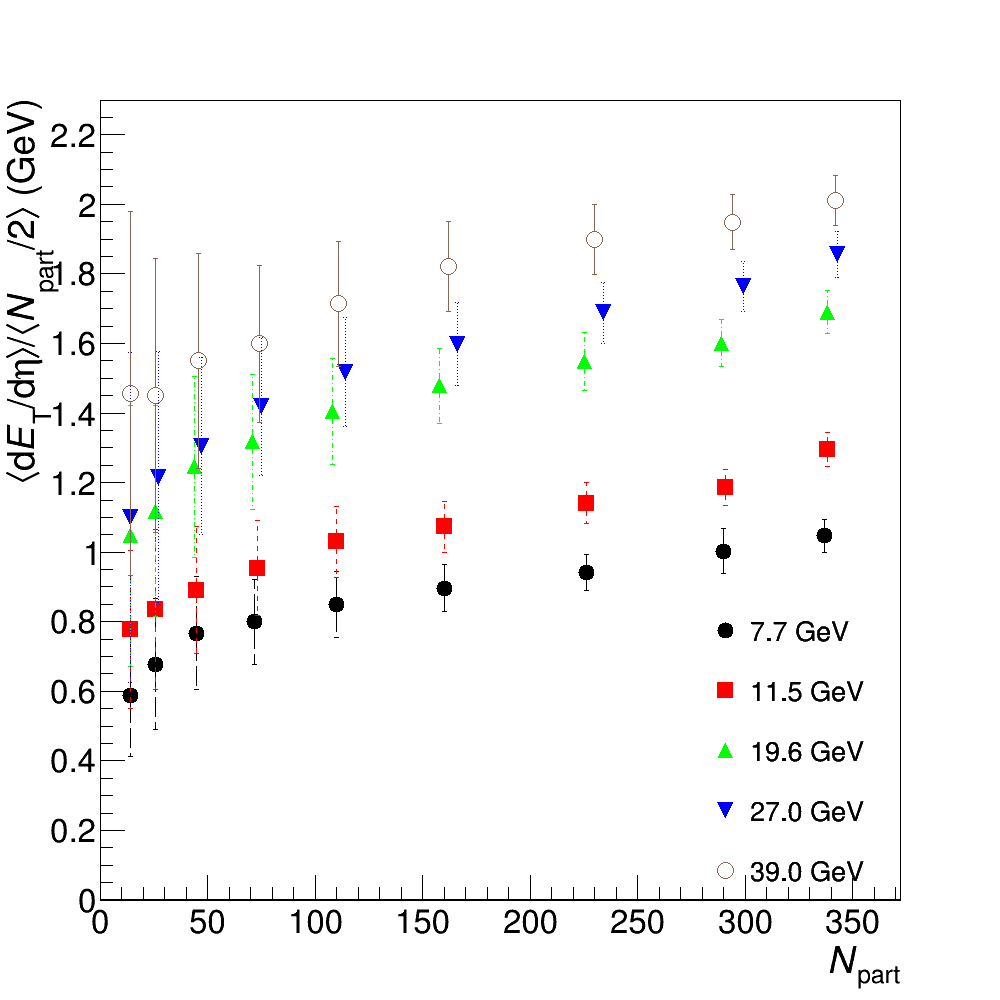
\includegraphics[width=5.5in]{{figures/finalStacked/dETdEtaOverNpartBy2SumEn39.0s}.png}
	  \caption{$(dE_{T}/d\eta)/0.5N_{part}$ at midrapidity as a function of ${N_{part}}$ for different collision energies.}\label{fig:dETdEtaOverNpartBy2SumEn}
	\end{figure}
\clearpage
}
\afterpage{%
	\begin{figure}[h]
	  \centering
	  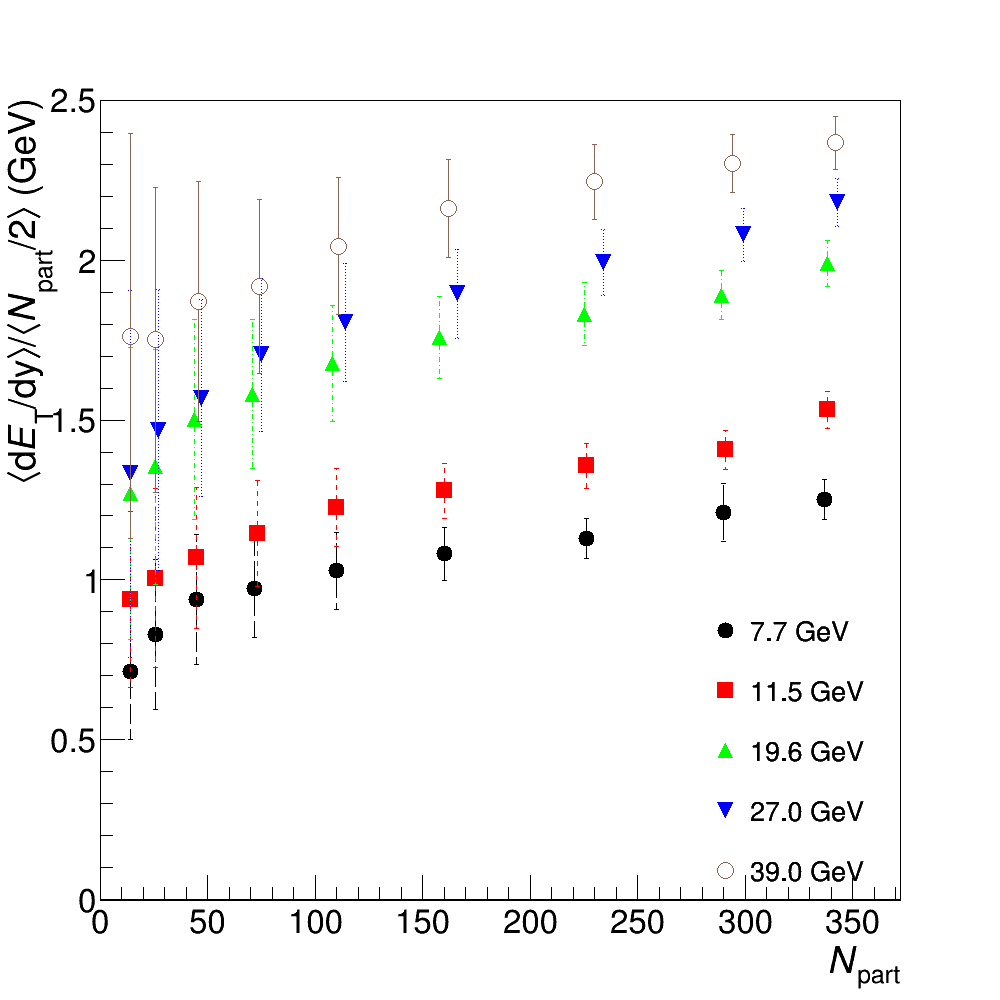
\includegraphics[width=5.5in]{{figures/finalStacked/dETdyOverNpartBy2SumEn39.0s}.png}
	  \caption{$(dE_{T}/dy)/0.5N_{part}$ at midrapidity as a function of ${N_{part}}$ for different collision energies.}\label{fig:dETdyOverNpartBy2SumEn}
	\end{figure}
\clearpage
}

Figure \ref{fig:dETdEtaOverdNchdEtaSumEn} shows the dependence of $E_{T}/N_{ch}$ on the number of nucleon participants. This ratio carries information about the average transverse mass of the final state particles produced from heavy ion collisions, and it has been found to not vary with the collision energy and centrality at RHIC energies \cite{PhysRevC.93.024901}. The results of this analysis show that this ratio remains roughly the same at higher values of $N_{part}$ but tends to grow smaller with decreasing $N_{part}$, albeit within the error bounds. It is also seen to increase with increasing collision energy. Figure \ref{fig:dETdyOverdNchdySumEn} is similar to Fig. \ref{fig:dETdEtaOverdNchdEtaSumEn} but in rapidity instead of pseudorapidity coordinates. The distributions show a similar trend although with some upward shift.
\afterpage{%
	\begin{figure}[h]
	  \centering
	  \includegraphics[width=5.5in]{{figures/finalStacked/dETdEtaOverdNchdEtaSumEn39.0s}.png}
	  \caption{$(dE_{T}/d\eta)/(dN_{ch}/d\eta)$ at midrapidity as a function of ${N_{part}}$ for different collision energies.}\label{fig:dETdEtaOverdNchdEtaSumEn}
	\end{figure}
\clearpage
}

\afterpage{%	
	\begin{figure}[h]
	  \centering
	  \includegraphics[width=5.5in]{{figures/finalStacked/dETdyOverdNchdySumEn39.0s}.png}
	  \caption{$(dE_{T}/dy)/(dN_{ch}/dy)$ at midrapidity as a function of ${N_{part}}$ for different collision energies.}\label{fig:dETdyOverdNchdySumEn}
	\end{figure}
\clearpage
}
%%%%%%%%%% snn plots:
%%%%%%%%%%%%%%%%%%%%%%%%%%%%%%%%%%%%%%%%%%%%%%%%%%%%%%%%%%%	
Figure \ref{fig:dETdEtaOverNpartBy2SumCents} shows the normalized $E_{T}$ as a function of collision energy for all the different collision centralities. This quantity increases with increasing collision energy and centrality while staying within the error bounds of the closest neighboring centralities. The slope of the distribution does not seem to vary a lot between centralities. Figure \ref{fig:dETdyOverNpartBy2SumCents} is similar to Fig. \ref{fig:dETdEtaOverNpartBy2SumCents} but in rapidity instead of pseudorapidity coordinates.
\afterpage{%
	\begin{figure}[h]
	  \centering
	  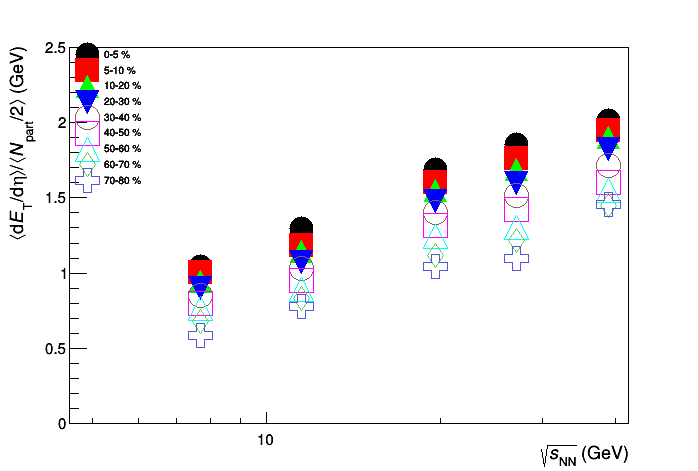
\includegraphics[width=5.5in]{figures/finalStacked/dETdEtaOverNpartBy2SumCent8s.png}
	  %\caption{$(dE_{T}/d\eta)/0.5N_{part}$ at midrapidity as a function of $\sqrt{s_{NN}}$ in logarithmic scale for different centralities. The dashed line represents a power-law fit to the 0-5\% central data in the form $y = ax^{2b}$, where $x$ and $y$ are the placeholders for the quantities in the plot axes. $\chi^{2}/n.d.f$ for the fit was 1.806, and the good-fit parameters were $a = 0.4838 \pm 0.0429$ and $b = 0.2005 \pm 0.01466$. The shaded area represents the uncertainty bounds for the 0-5\% central PHENIX data from \cite{PhysRevC.93.024901}. }\label{fig:dETdEtaOverNpartBy2SumCents}
	  \caption{$(dE_{T}/d\eta)/0.5N_{part}$ at midrapidity as a function of $\sqrt{s_{NN}}$ in logarithmic scale for different centralities.}\label{fig:dETdEtaOverNpartBy2SumCents}
	\end{figure}
\clearpage
}
\afterpage{%
	\begin{figure}[h]
	  \centering
	  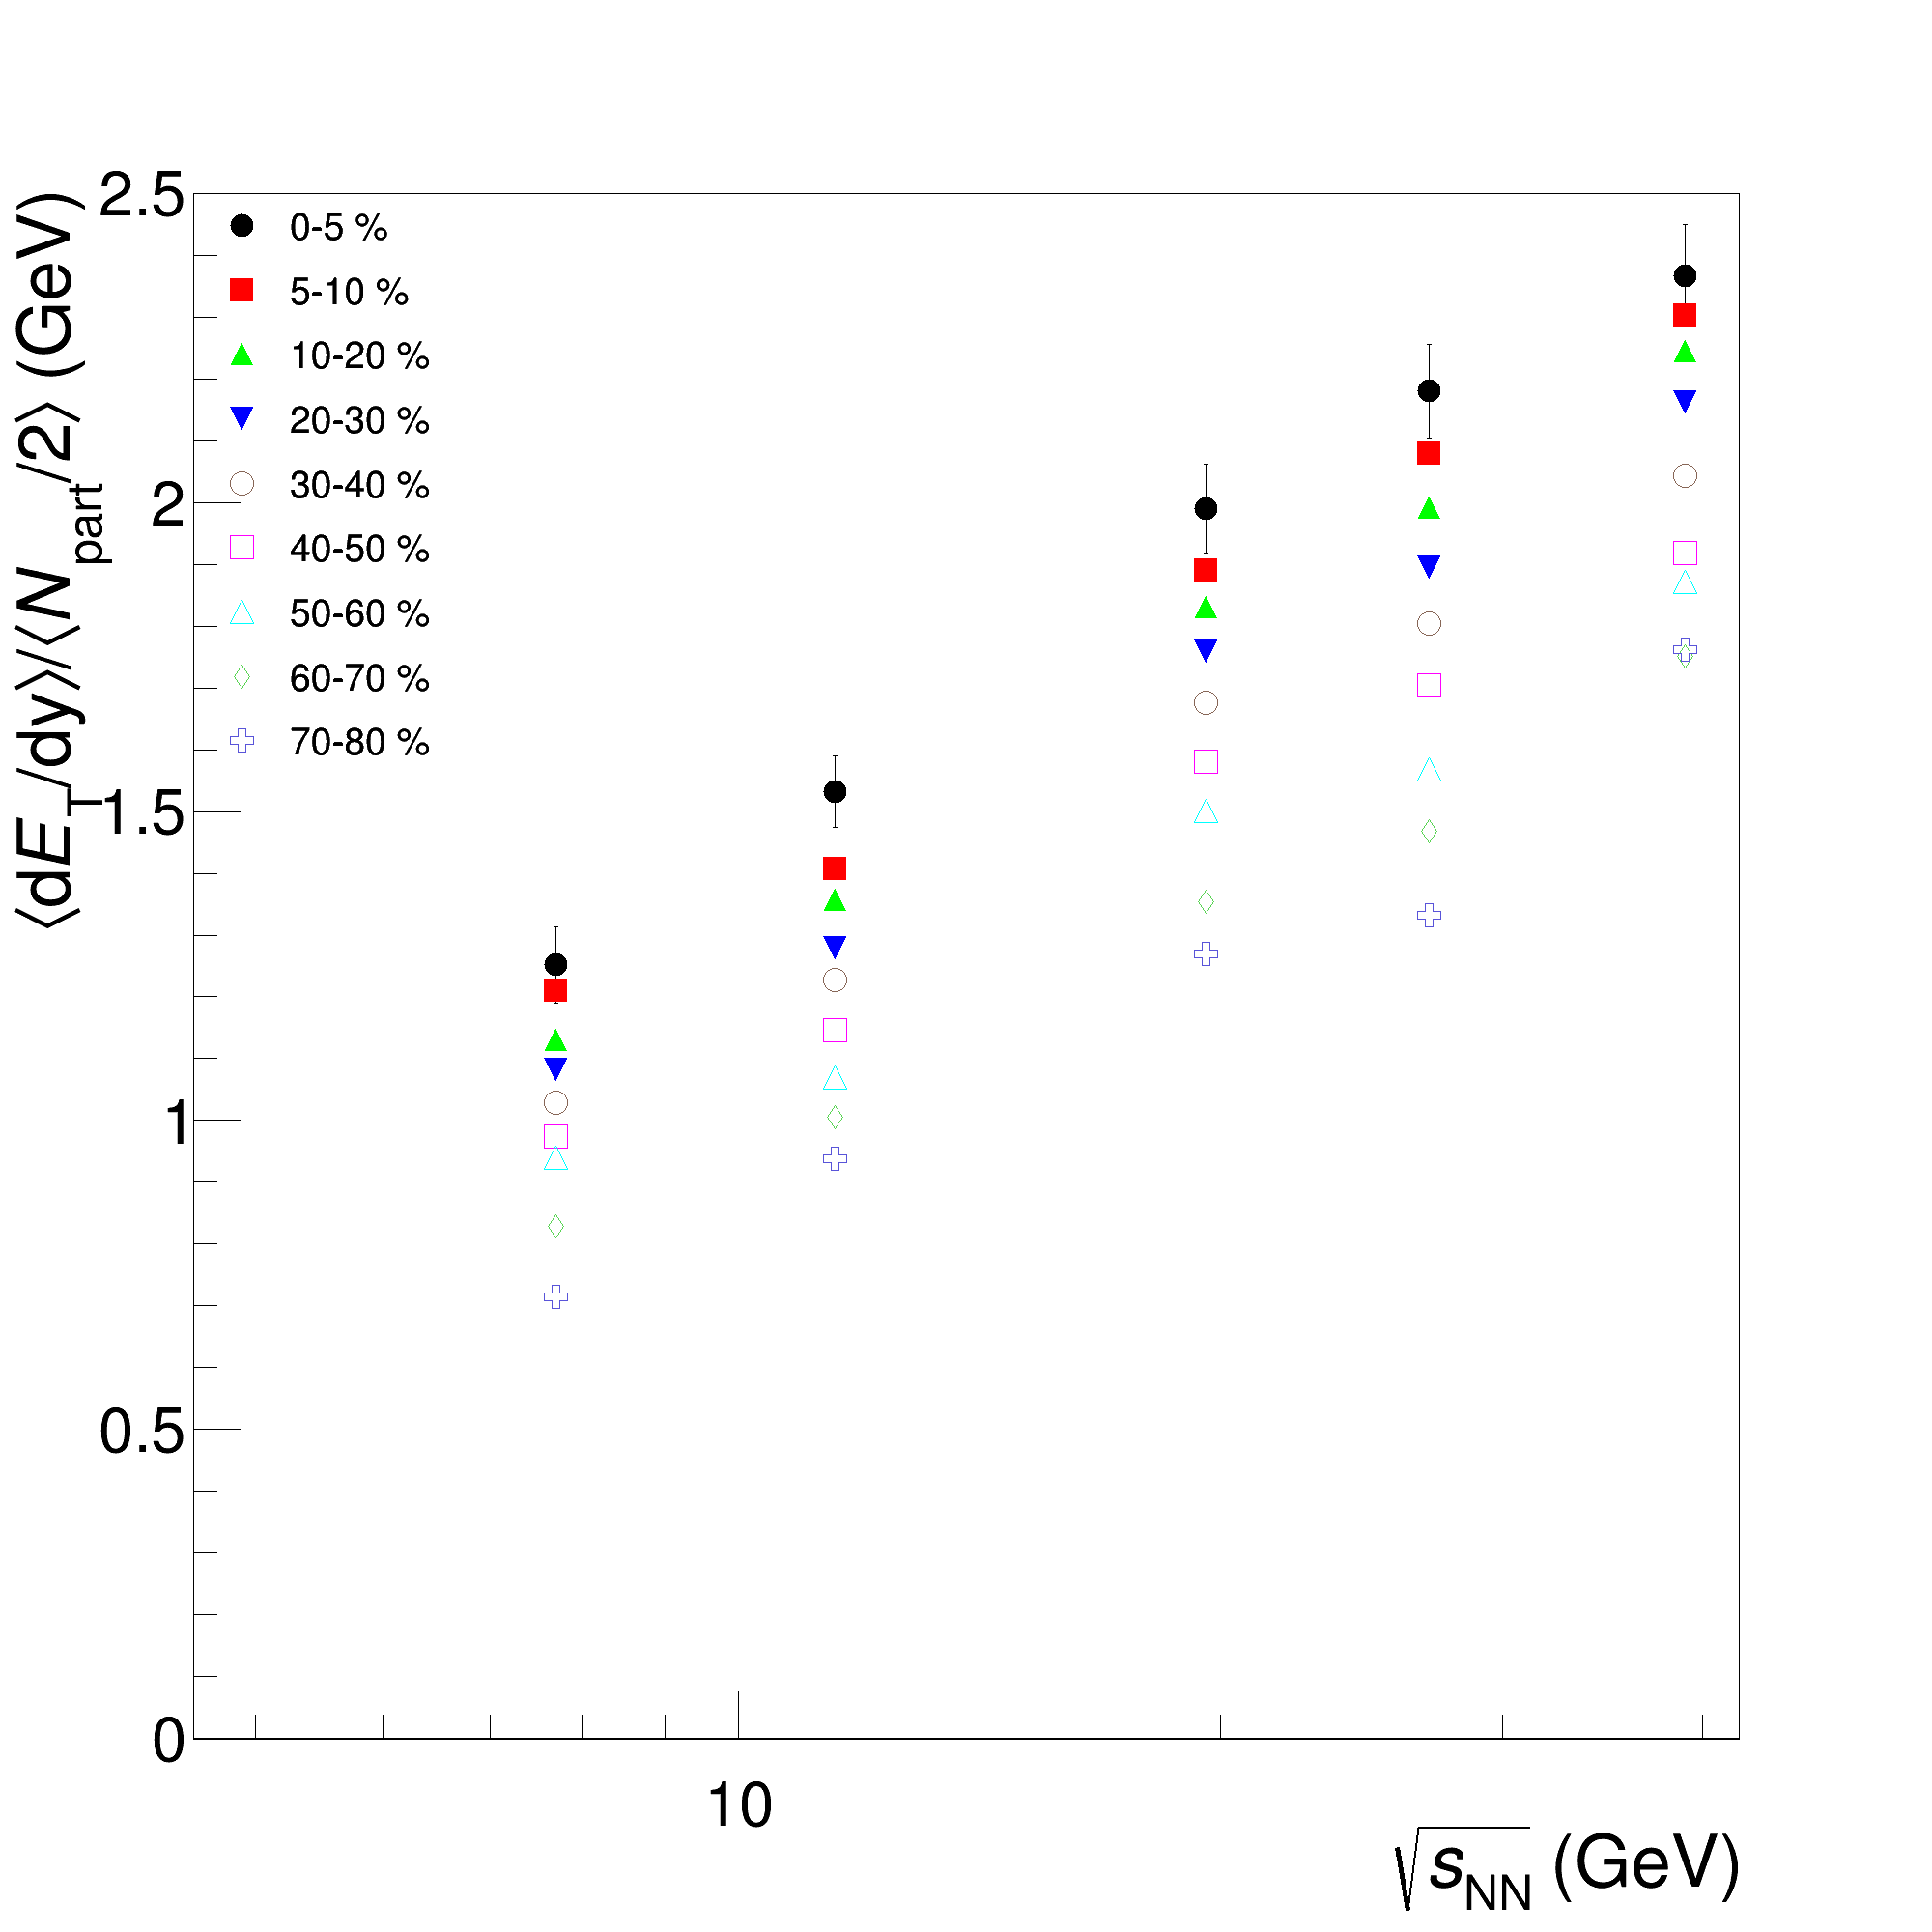
\includegraphics[width=5.5in]{figures/finalStacked/dETdyOverNpartBy2SumCent8s.png}
	  \caption{$(dE_{T}/dy)/0.5N_{part}$ at midrapidity as a function of $\sqrt{s_{NN}}$ for different centralities.}\label{fig:dETdyOverNpartBy2SumCents}
	\end{figure}
\clearpage
}
%%%%%%%%%%%%%%
Figures \ref{fig:dETdEtaOverdNchdEtaSumCents} and \ref{fig:dETdyOverdNchdySumCents} show the dependence of $E_{T}/N_{ch}$ on the collision energy in, respectively, pseudorapidity and rapidity coordinates. The $\sqrt{s_{NN}}$ axis is again in logarithmic scale. The ratio $E_{T}/N_{ch}$ increases with increasing collision energy. The slope of the distributions seem to decrease with increasing centrality for the more central collisions.	The more central collisions also show fluctuations in the way $E_{T}/N_{ch}$ increases as a function of $\sqrt{s_{NN}}$.
	
\afterpage{%
	\begin{figure}[h]
	  \centering
	  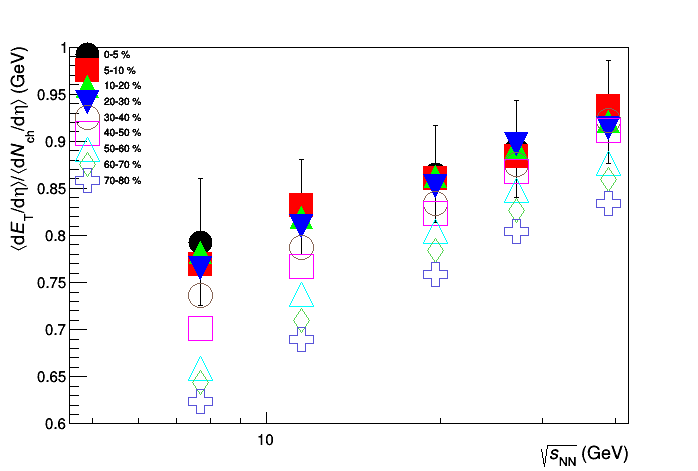
\includegraphics[width=5.5in]{figures/finalStacked/dETdEtaOverdNchdEtaSumCent8s.png}
	  \caption{$(dE_{T}/d\eta)/(dN_{ch}/d\eta)$ at midrapidity as a function of $\sqrt{s_{NN}}$ for different centralities.}\label{fig:dETdEtaOverdNchdEtaSumCents}
	\end{figure}
\clearpage
}	
\afterpage{%
	\begin{figure}[h]
	  \centering
	  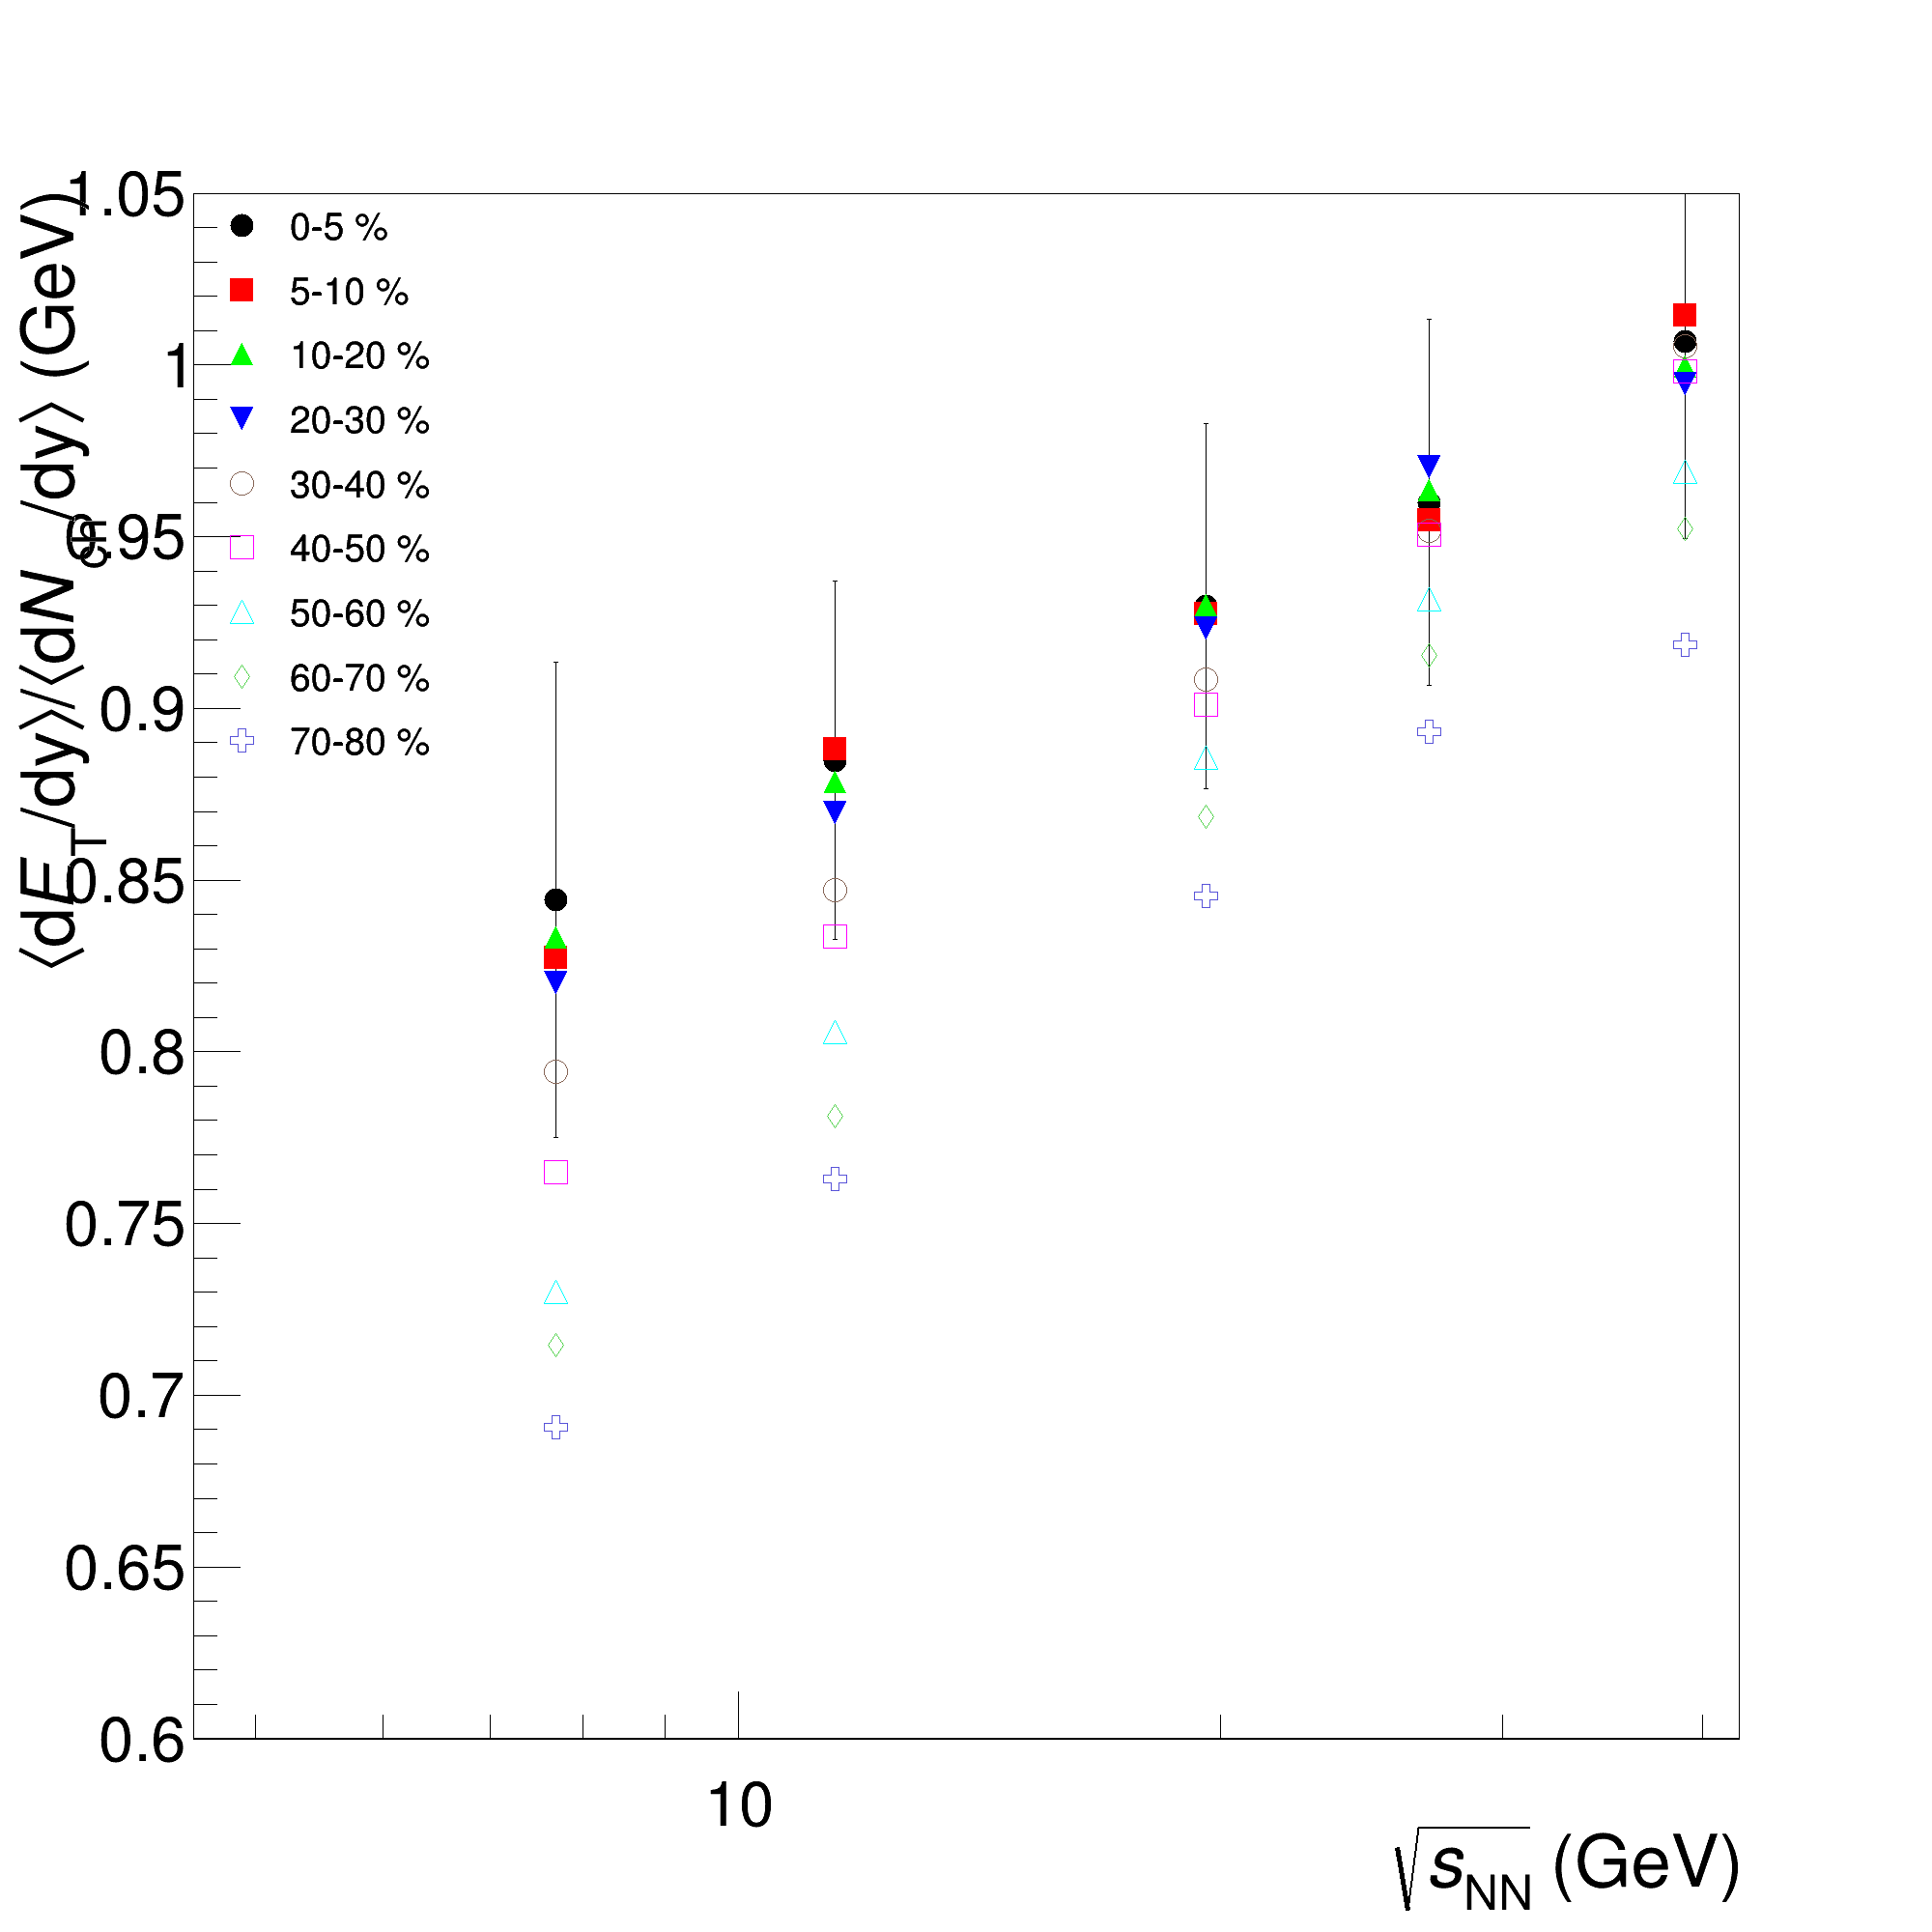
\includegraphics[width=5.5in]{figures/finalStacked/dETdyOverdNchdySumCent8s.png}
	  \caption{$(dE_{T}/dy)/(dN_{ch}/dy)$ at midrapidity as a function of $\sqrt{s_{NN}}$ for different centralities.}\label{fig:dETdyOverdNchdySumCents}
	\end{figure}
\clearpage
}

% comparison with Adare et al.
Figure \ref{fig:comparison} puts the 0-5\% collision results of this analysis in perspective with the result from \cite{PhysRevC.93.024901} based on PHENIX calorimetry. The normalized $E_{T}$ from this analysis is higher than that from PHENIX for all the available collision energies. The $(dE_{T}/dy)/0.5N_{part}$ values for $\sqrt{s_{NN}}$ = 7.7, 19.6, 27, and 39 GeV are found to differ by 2.82, 2.83, 2.37 and 1.67 standard deviations respectively. Since these two measurements are truly independent and the calculated deviations aren't too extreme, this may just reflect a tension between STAR and PHENIX. There may also be a slight effect due to the difference in the rapidity ranges corresponding to the two different measurements, as well as the different sensitivities in the methods to estimate particle compositions and Monte Carlo generators used for corrections. The next step is to make similar comparisons in the collision energy regimes where identified particle spectra are available from both experiments, but that is out of the scope of this thesis.%  The explanation of these differences require a meticulous analysis of the assumptions made by both measurements and is left for future work. 

\afterpage{%
	\begin{figure}[h]
	  \centering
	  \includegraphics[width=4.5in]{figures/PHENIX_comparison2.png}
	  \caption{$\frac{dE_{T}}{d\eta}/0.5N_{part}$ for 0-5\% central collisions at midrapidity as a function of $\sqrt{s_{NN}}$. The PHENIX data are from \cite{PhysRevC.93.024901}. The error bars represent the total statistical and systematic uncertainties.}\label{fig:comparison}
	\end{figure}
\clearpage
}	
	
	
%cnt97kx Send this link to your invitees ... http://whenisgood.net/fndqz2a This is where your results will appear ... http://whenisgood.net/fndqz2a/results/cnt97kx And use this link to edit your event ... http://whenisgood.net/fndqz2a/edit/cnt97kx

    \include{chapters/chapter-7}
    \include{chapters/chapter-8}
    \include{chapters/chapter-9}
    \include{chapters/chapter-10}
    \include{back-matter}
    %%%%%%%%%%%%%%%%%%%%%%%%%%%%%%%%%%%%%%%%%%%%%%%%%%%%%%%%%%%%%%%%%%%%%%%%%%%%%%%%%%%%%%%%%%%%%%%%%%%%%
    % BIBLIOGRAPHY
    %%%%%%%%%%%%%%%%%%%%%%%%%%%%%%%%%%%%%%%%%%%%%%%%%%%%%%%%%%%%%%%%%%%%%%%%%%%%%%%%%%%%%%%%%%%%%%%%%%%%%
    \makeBibliographyPage % make the bibliography title page
\newpage

% To make the bibliography, use \utbiblio{#1}{}{} command. Always use "#1" for the first entry. The second entry is your bibliography style, and the third entry is the name of your bibliography file (.bib file extension) 
% bibliography style - recommend using apalike-doi as it hyperlinks DOIs
% Be sure to run BibTeX in order to generate the bibliography correctly.

\utbiblio{#1}{apsrev}{references-Biswas}

    %%%%%%%%%%%%%%%%%%%%%%%%%%%%%%%%%%%%%%%%%%%%%%%%%%%%%%%%%%%%%%%%%%%%%%%%%%%%%%%%%%%%%%%%%%%%%%%%%%%%%
    % APPENDIX - OPTIONAL - COMMENT OUT IF NOT NEEDED
    %%%%%%%%%%%%%%%%%%%%%%%%%%%%%%%%%%%%%%%%%%%%%%%%%%%%%%%%%%%%%%%%%%%%%%%%%%%%%%%%%%%%%%%%%%%%%%%%%%%%%
    
    \makeAppendixPage{1}   % Input the number of appendices
    \appendix    
    \include{back-matter/appendix-1}
    %\include{back-matter/appendix-2}
    %%%%%%%%%%%%%%%%%%%%%%%%%%%%%%%%%%%%%%%%%%%%%%%%%%%%%%%%%%%%%%%%%%%%%%%%%%%%%%%%%%%%%%%%%%%%%%%%%%%%%
    % A VITA IS REQUIRED
    %%%%%%%%%%%%%%%%%%%%%%%%%%%%%%%%%%%%%%%%%%%%%%%%%%%%%%%%%%%%%%%%%%%%%%%%%%%%%%%%%%%%%%%%%%%%%%%%%%%%%
    \addToTOC{Vita}
    \chapter*{Vita}
Biswas Sharma was born in Kathmandu, Nepal to the parents of Byas and Manju Sharma. He has a younger sibling: Binamrata Sharma. He graduated from high school at St. Xavier's College, Kathmandu. He graduated with a BS in Astrophysics and a BS in Mathematics from Morehead State University, Kentucky in 2015. He graduated with a masters in Physics from The University of Tennessee, Knoxville, in Summer, 2018.

\end{document}
